\section{Computationally Cheap Acquisition Functions}
%----------------------------------------------------------------------
%----------------------------------------------------------------------
\begin{frame}[c]{Acquisition Functions}
\framesubtitle{Description}
\begin{itemize}
    \item \emph{Problem:} Given the surrogate function $\iter{\surro}$ at the $\bocount\,$th iteration of BO, choose the "best" candidate $\iter{\conf}\in \pcs$ to evaluate $\cost$ at next
    \pause
    \smallskip
    \item \emph{Solution(?):} Evaluate at a global minimum of $\iter{\surro}$ 
    \item \emph{Issues:}
    \begin{itemize}
        \item The surrogate function is inaccurate. The global optimum of $\iter{\surro}$ does not necessarily yield the \emph{best} $\cost(\conf)$. 
        \item Considering our uncertainty in the surrogate model, we also need to \emph{trade off exploration and exploitation}
    \end{itemize}
    \pause
    \item \emph{Real Solution}: Use a heuristic utility function $\acq(\cdot)$ aka \emph{acquisition function} that trades off exploration and exploitation!
\end{itemize}

\end{frame}
%-----------------------------------------------------------------------
\begin{frame}[t]{Computationally Cheap Acquisition Functions - PI}
\framesubtitle{Probability of Improvement - Concept}
\begin{figure}
  \centering
  \begin{tikzpicture}
    \node<+> (img1) {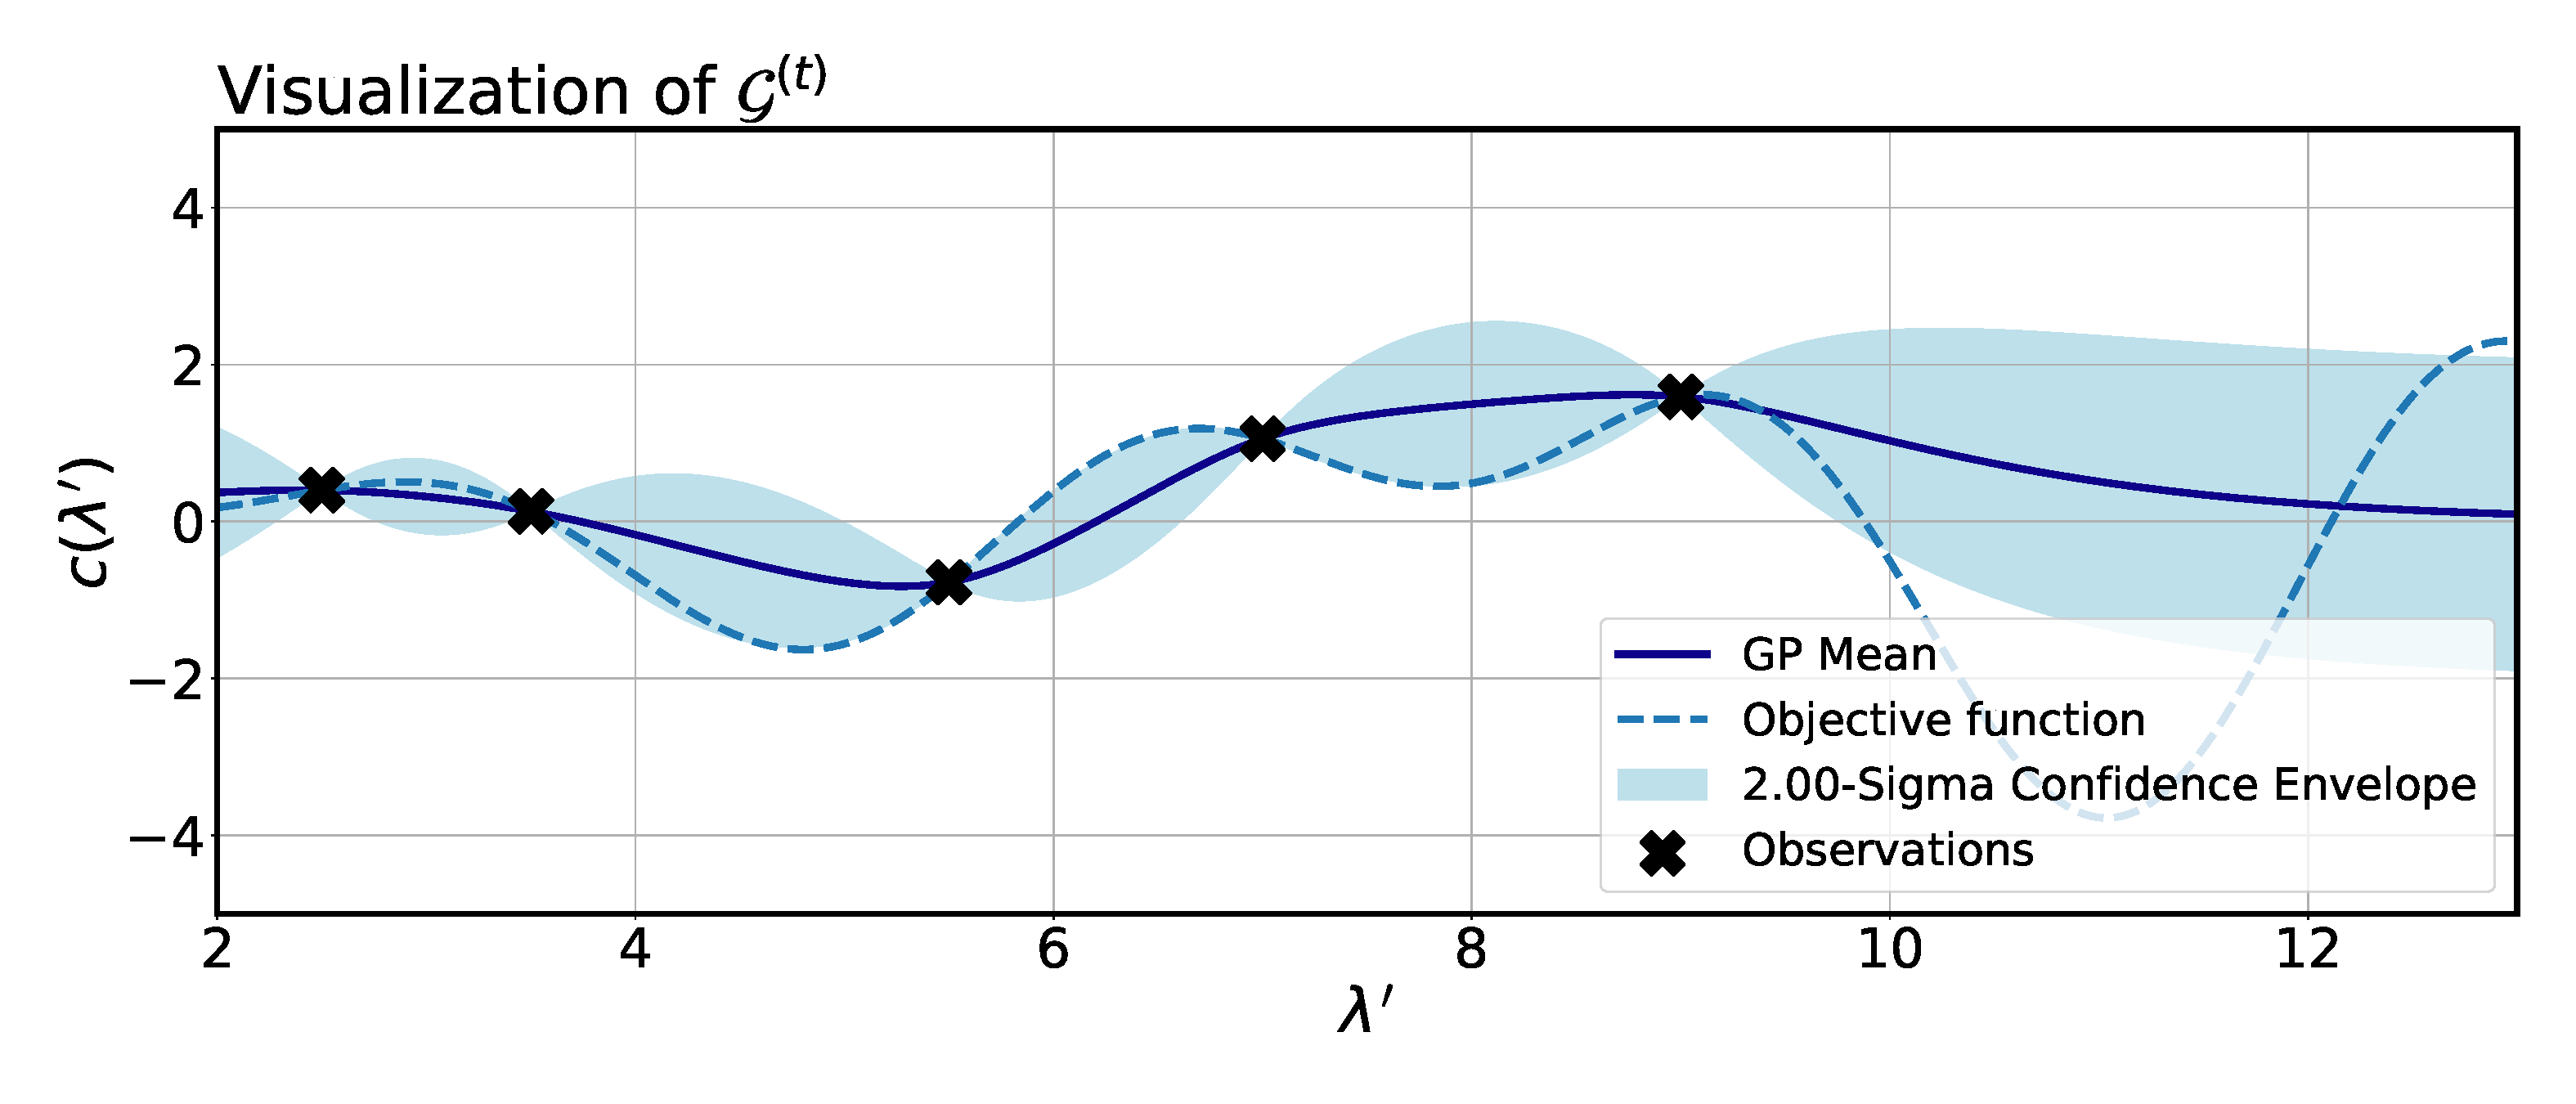
\includegraphics[width=\linewidth, height=0.7\textheight, keepaspectratio=true]{images/acq_func_images/pi/pi_1.pdf}};
    \node<.> [below=0.01\belowcaptionskip of img1, align=center]{Given the GP at iteration $\bocount$ fit on dataset $\iter[\bocount-1]{\dataset}$};

    \node<+> (img2) {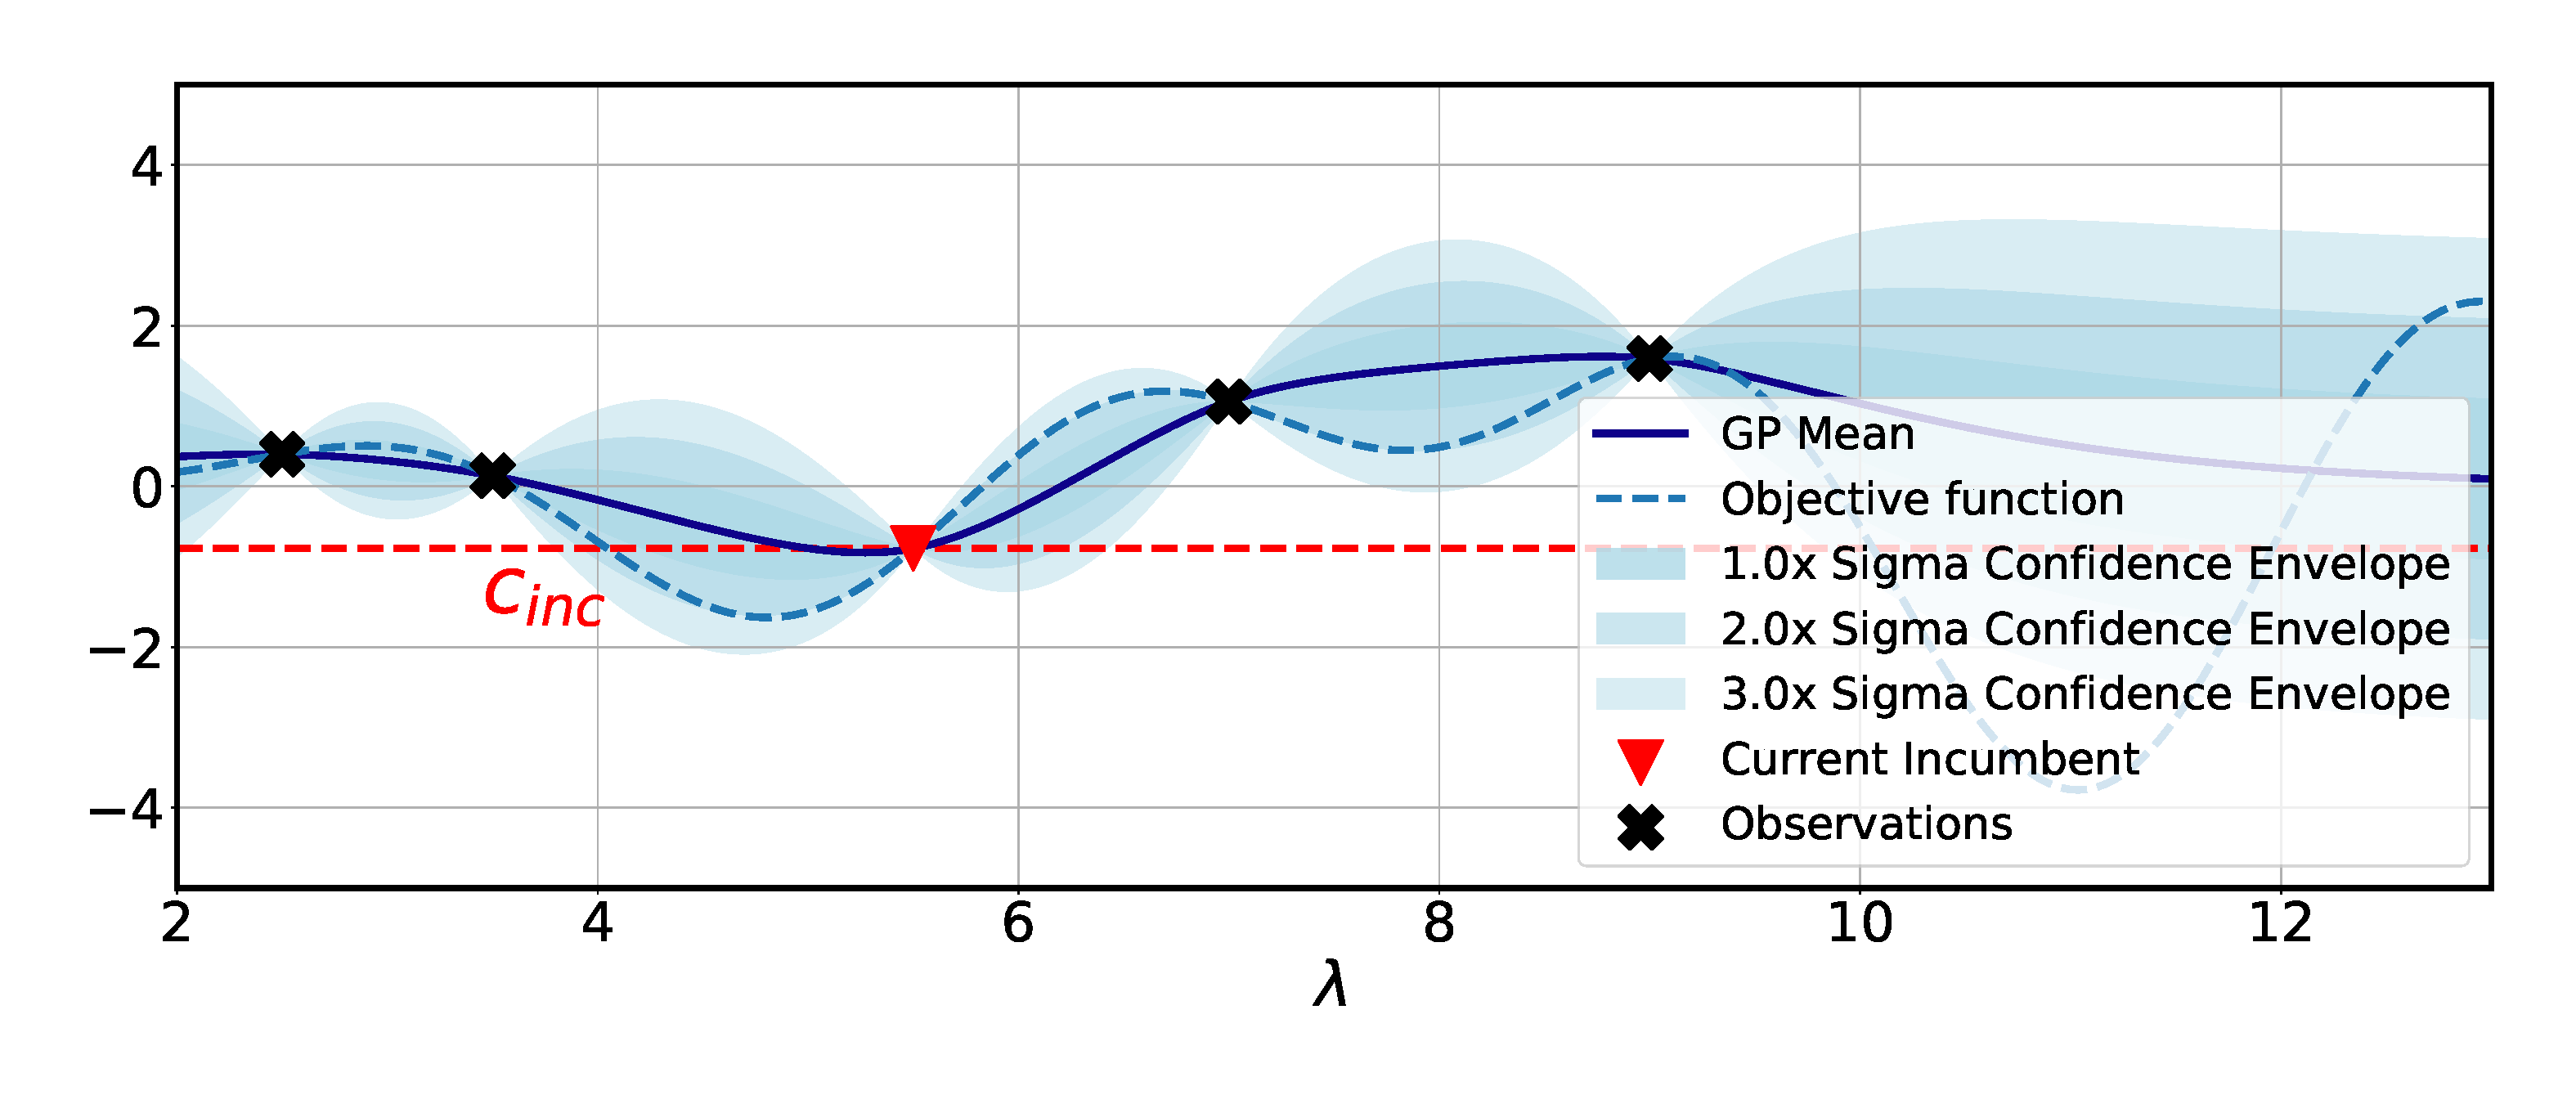
\includegraphics[width=\linewidth, height=0.7\textheight, keepaspectratio=true]{images/acq_func_images/pi/pi_2.pdf}};
    \node<.> [below=0.01\belowcaptionskip of img2, align=center]{Current incumbent $\incumbent[\bocount-1]$ and its observed cost $\cost(\incumbent[\bocount-1])$};

    \node<+> (img3) {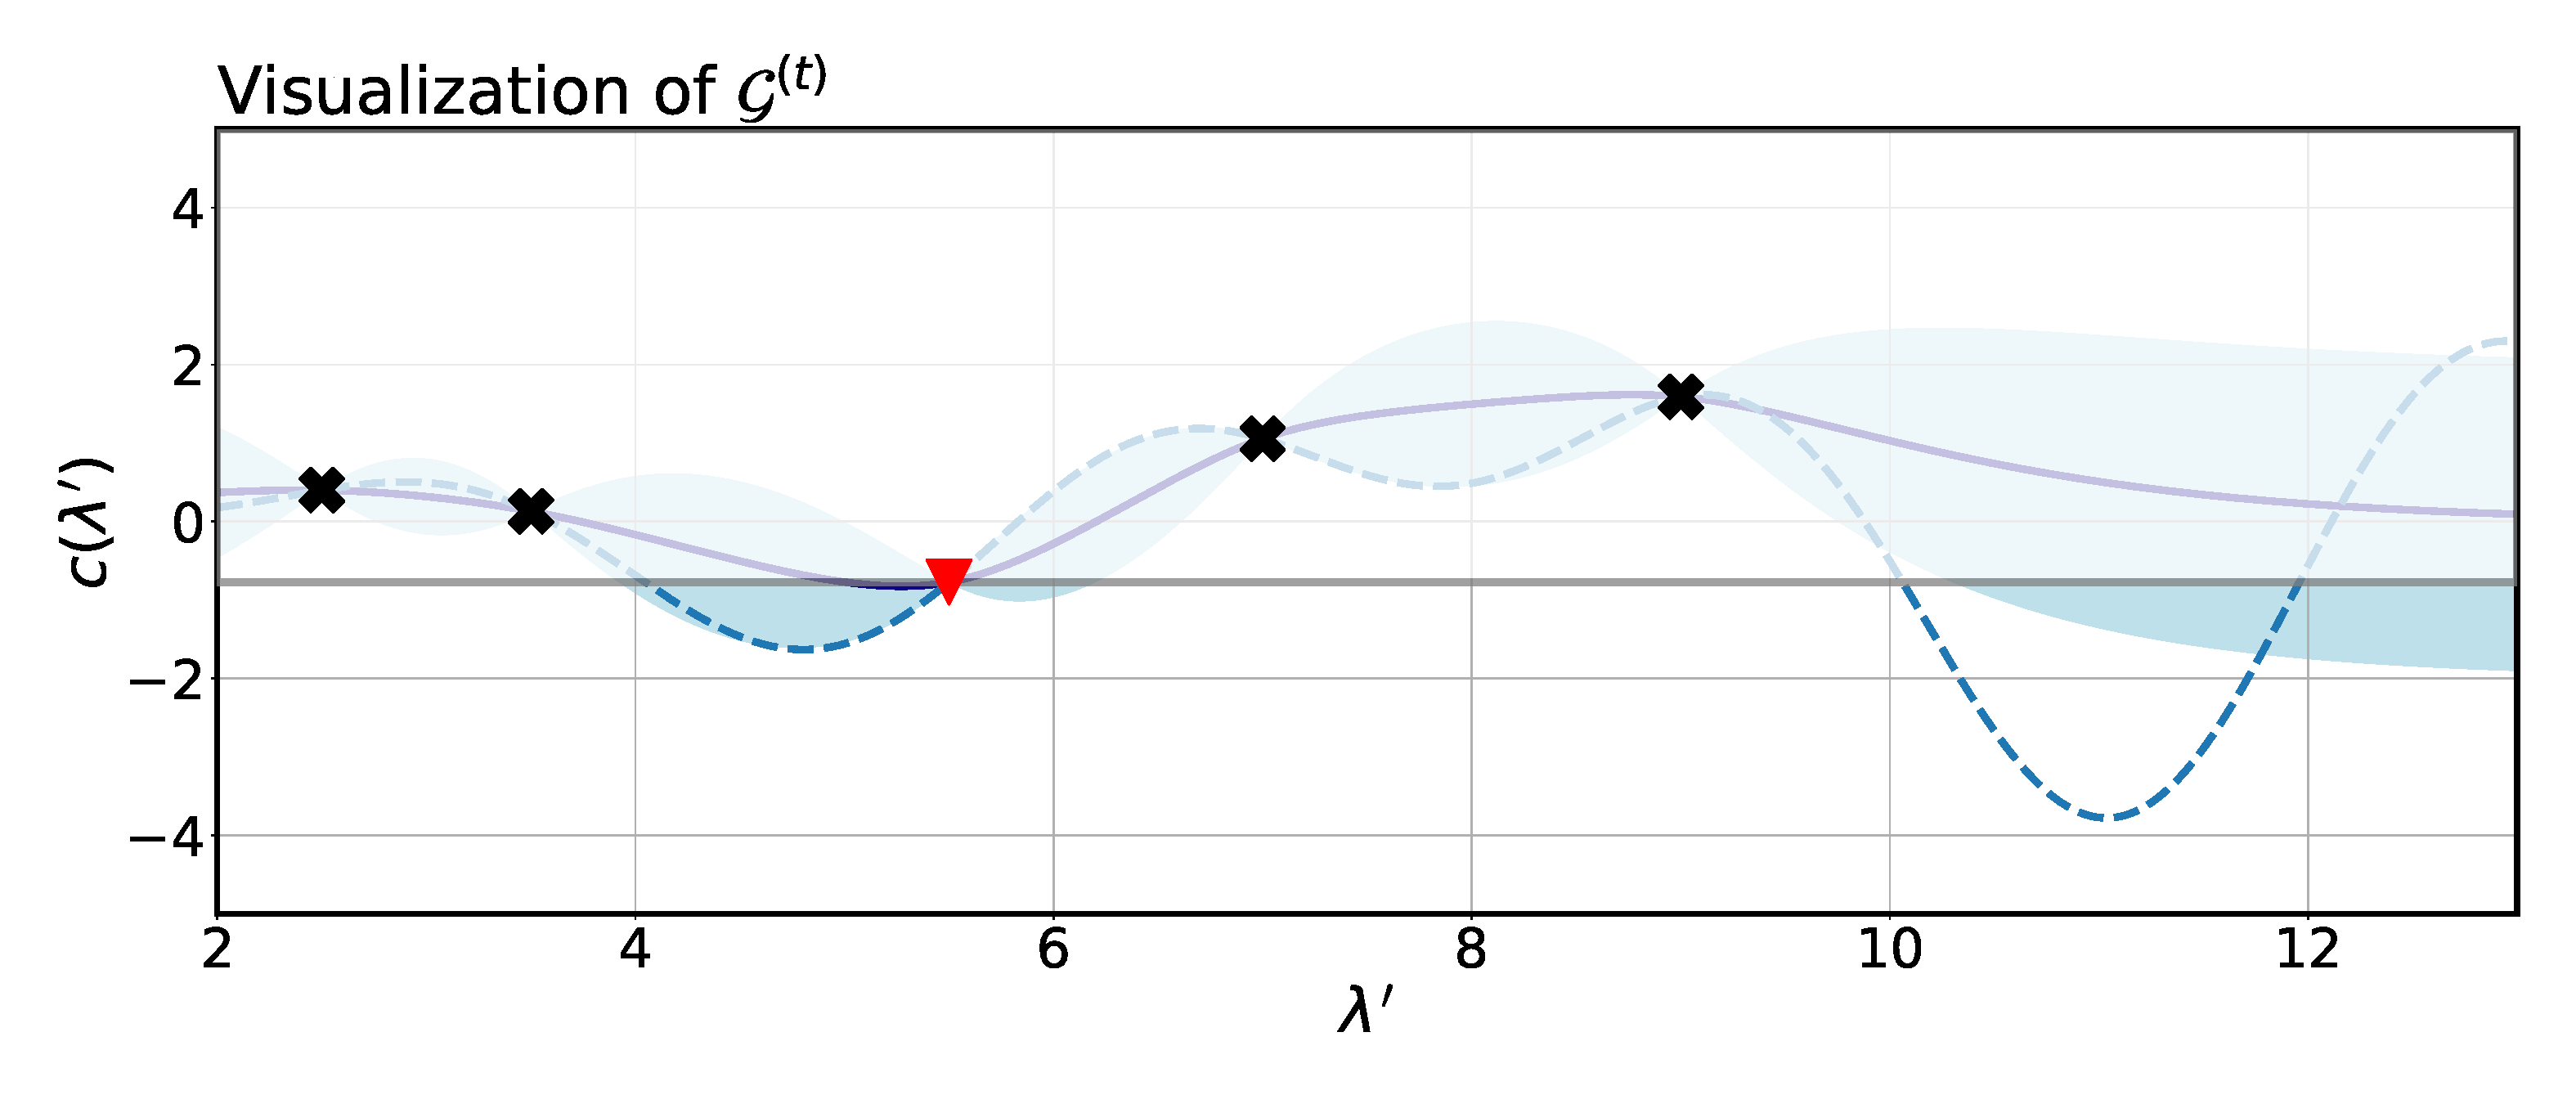
\includegraphics[width=\linewidth, height=0.7\textheight, keepaspectratio=true]{images/acq_func_images/pi/pi_3.pdf}};
    \node<.> [below=-1.0\belowcaptionskip of img3, align=center]{Intuitively, we can disregard the section of the search space with higher costs \\than our incumbent. Hence, we now only look at the \emph{Region of Probable Improvement}};
    \comment{We cannot be absolutely certain if there will be an improvement, but we are certain that if there is to be improvement, it is only possible in this zone.}

    \node<+> (img4) {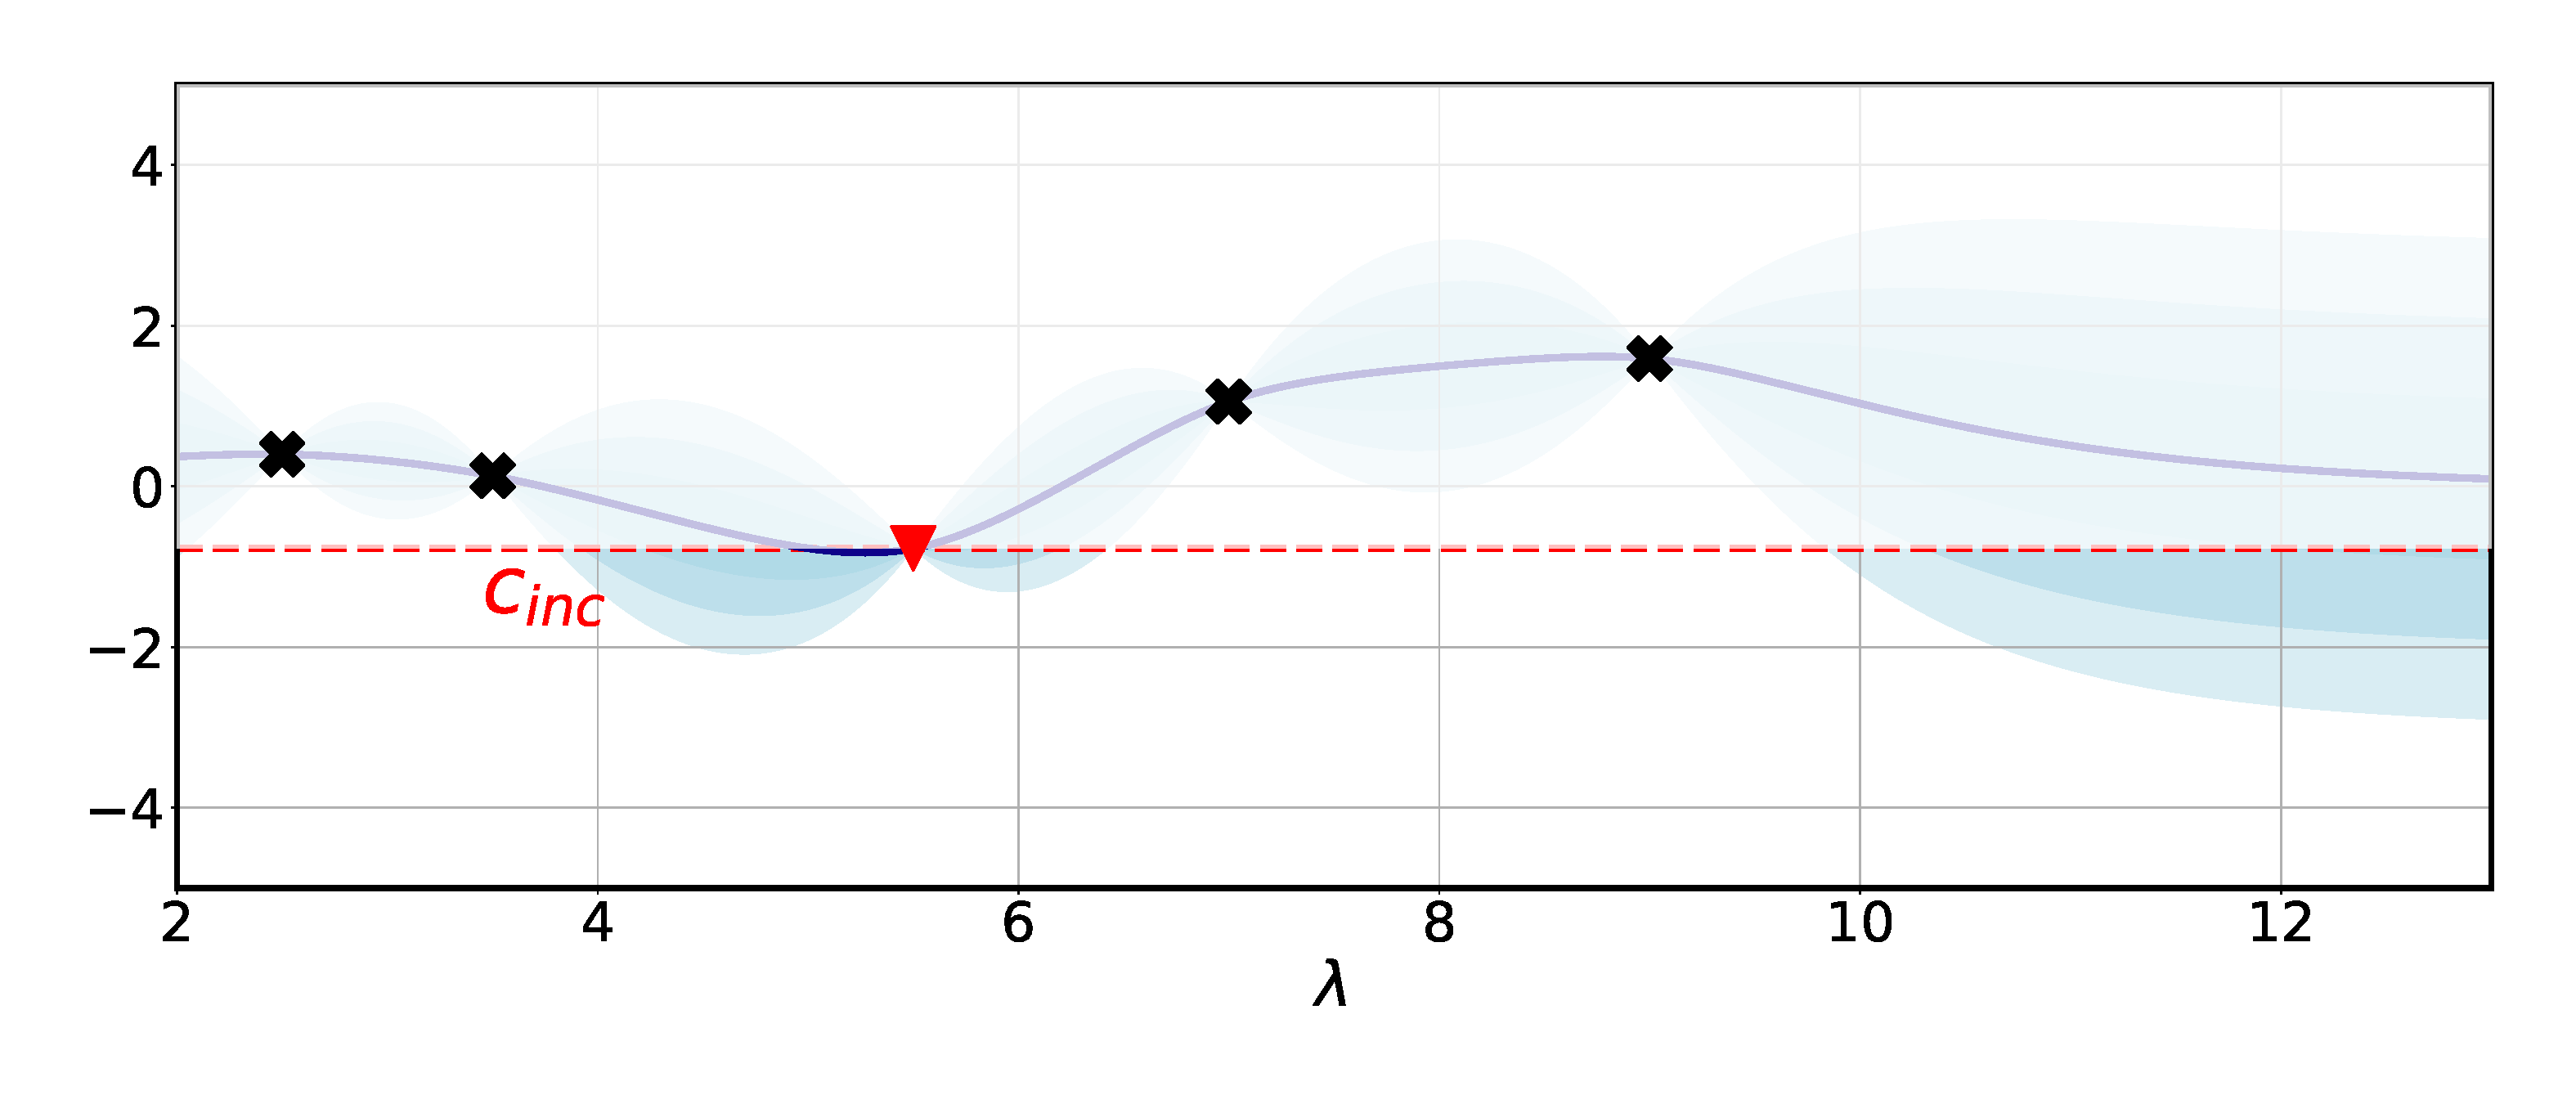
\includegraphics[width=\linewidth, height=0.7\textheight, keepaspectratio=true]{images/acq_func_images/pi/pi_4.pdf}};
    \node<.> [below=0.01\belowcaptionskip of img4, align=center]{PDF of a good candidate configuration. Only the green area is an improvement.};

    \node<+> (img5) {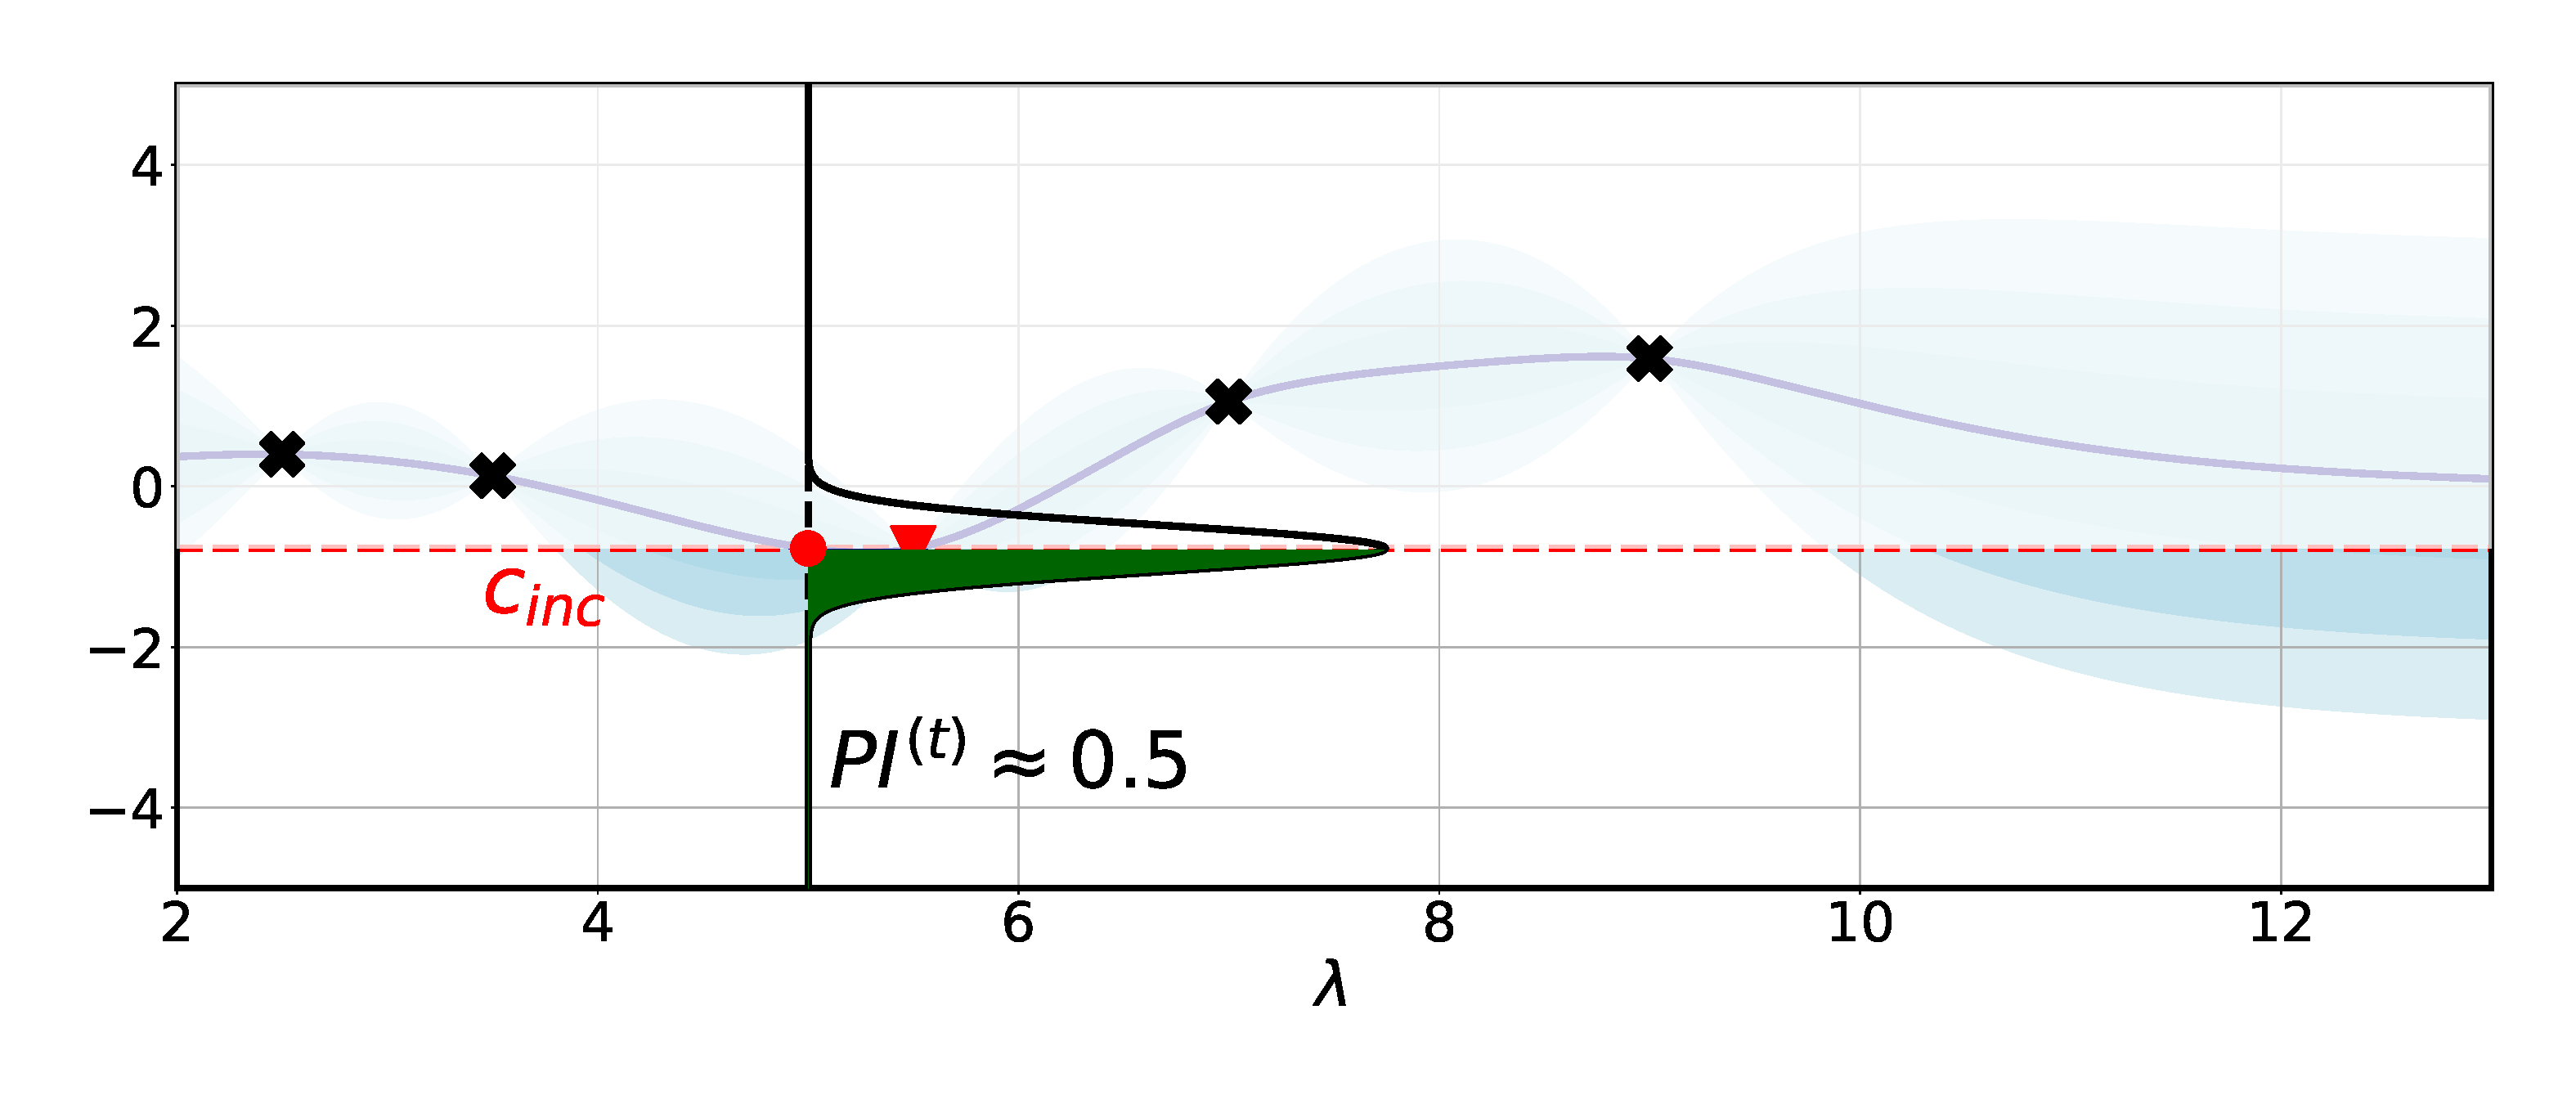
\includegraphics[width=\linewidth, height=0.7\textheight, keepaspectratio=true]{images/acq_func_images/pi/pi_5.pdf}};
    \node<.> [below=0.01\belowcaptionskip of img5, align=center]{PDF of a bad candidate configuration};
  \end{tikzpicture}
\end{figure}

\end{frame}
%-----------------------------------------------------------------------
\begin{frame}[c]{Computationally Cheap Acquisition Functions - PI}
\framesubtitle{Probability of Improvement - Choosing a candidate}
\comment{The definitions were adapted from the source to fit an acquisition function that is maximized and an objective function which is to be minimized.!}
\begin{itemize}
    \item[]
        \[
            \iter{\acq}_{PI}(\conf) = P(\cost(\conf) \leq \cost(\incumbent[\bocount-1])), \quad \text{where } \incumbent[\bocount-1]\in\argmin_{\conf'\in\iter[\bocount-1]{\dataset}}\obs[\conf']\in\iter[\bocount-1]{\dataset}
        \]
    \pause
    \bigskip
    \bigskip
    This can be written as:
    \vspace*{-1.0cm}
    \[
        \iter{\acq}_{PI}(\conf) = \cdf[Z], \quad \text{with } Z = \dfrac{\cost(\incumbent[\bocount-1]) - \iter[\bocount-1]{\mean}(\conf) - \xi}{\iter[\bocount-1]{\stddev}(\conf)}, 
    \]
    \newline
    where $\cdf(\cdot)$ is the CDF of the standard normal distribution and $\xi$ is an optional exploration parameter.
    \pause
    \item[] \[\boxed{\text{Choose } \bonextsample \in \argmax_{\conf\in\pcs}(\iter{\acq}_{PI}(\conf))}\]
%    \comment{Source: Tutorial by Brochu et al.: https://arxiv.org/pdf/1012.2599.pdf }
\end{itemize}
\end{frame}
%-----------------------------------------------------------------------
\begin{frame}[t]{Computationally Cheap Acquisition Functions - EI}
\framesubtitle{Expected Improvement - Concept}

\begin{figure}
  \centering
  \begin{tikzpicture}
    \node<+> (img1) {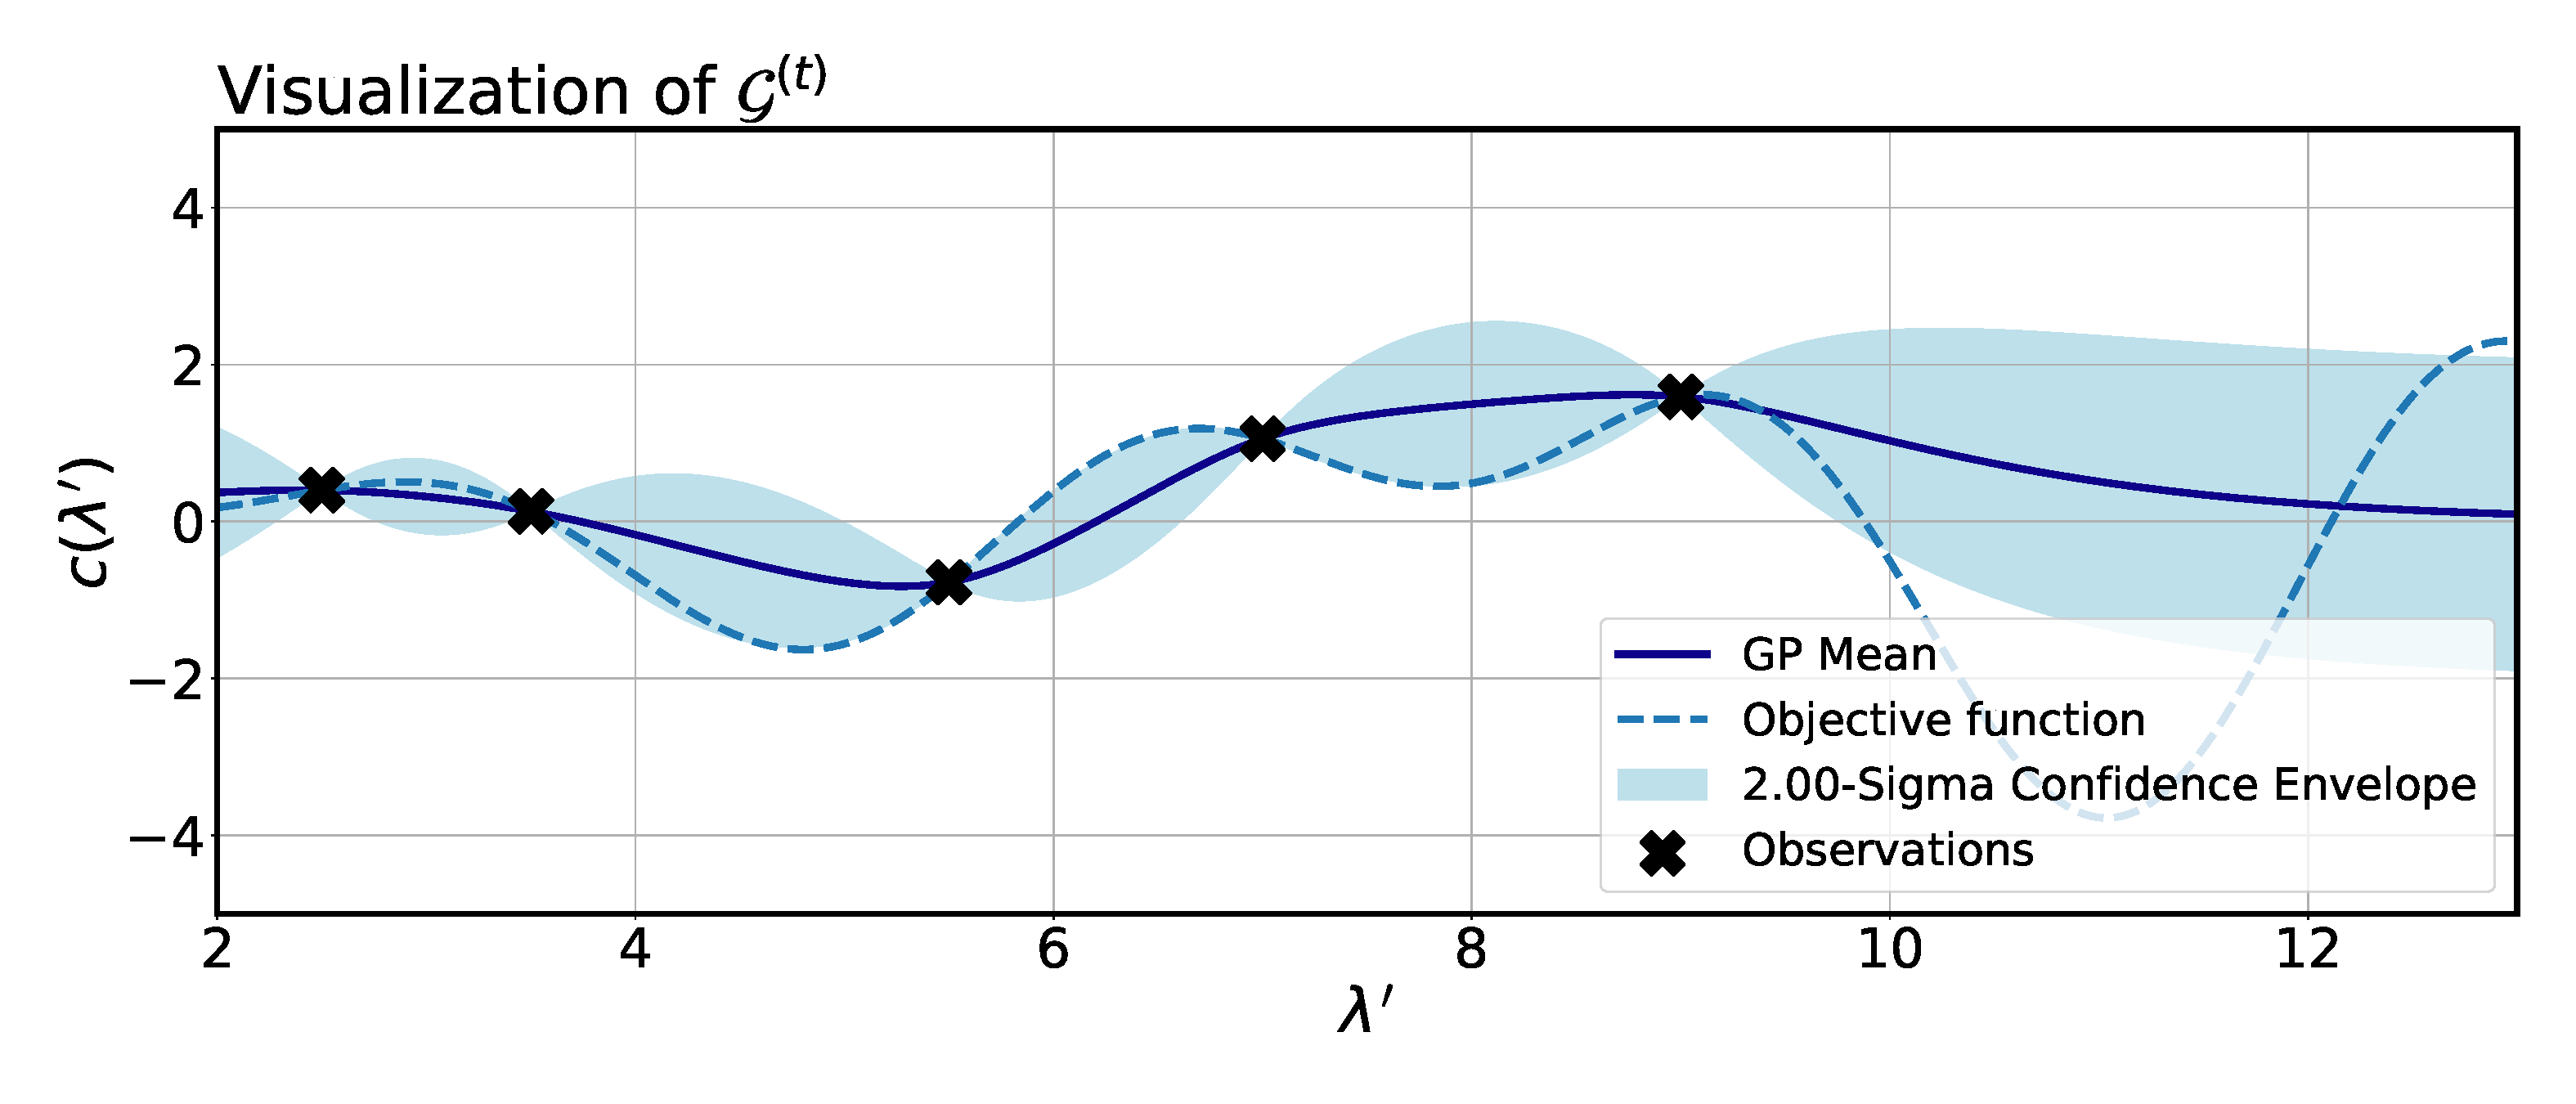
\includegraphics[width=\linewidth, height=0.7\textheight, keepaspectratio=true]{images/acq_func_images/ei/ei_1.pdf}};
    \node<.> [below=0.01\belowcaptionskip of img1, align=center]{Given the GP at iteration $\bocount$ fit on dataset $\iter[\bocount-1]{\dataset}$};

    \node<+> (img2) {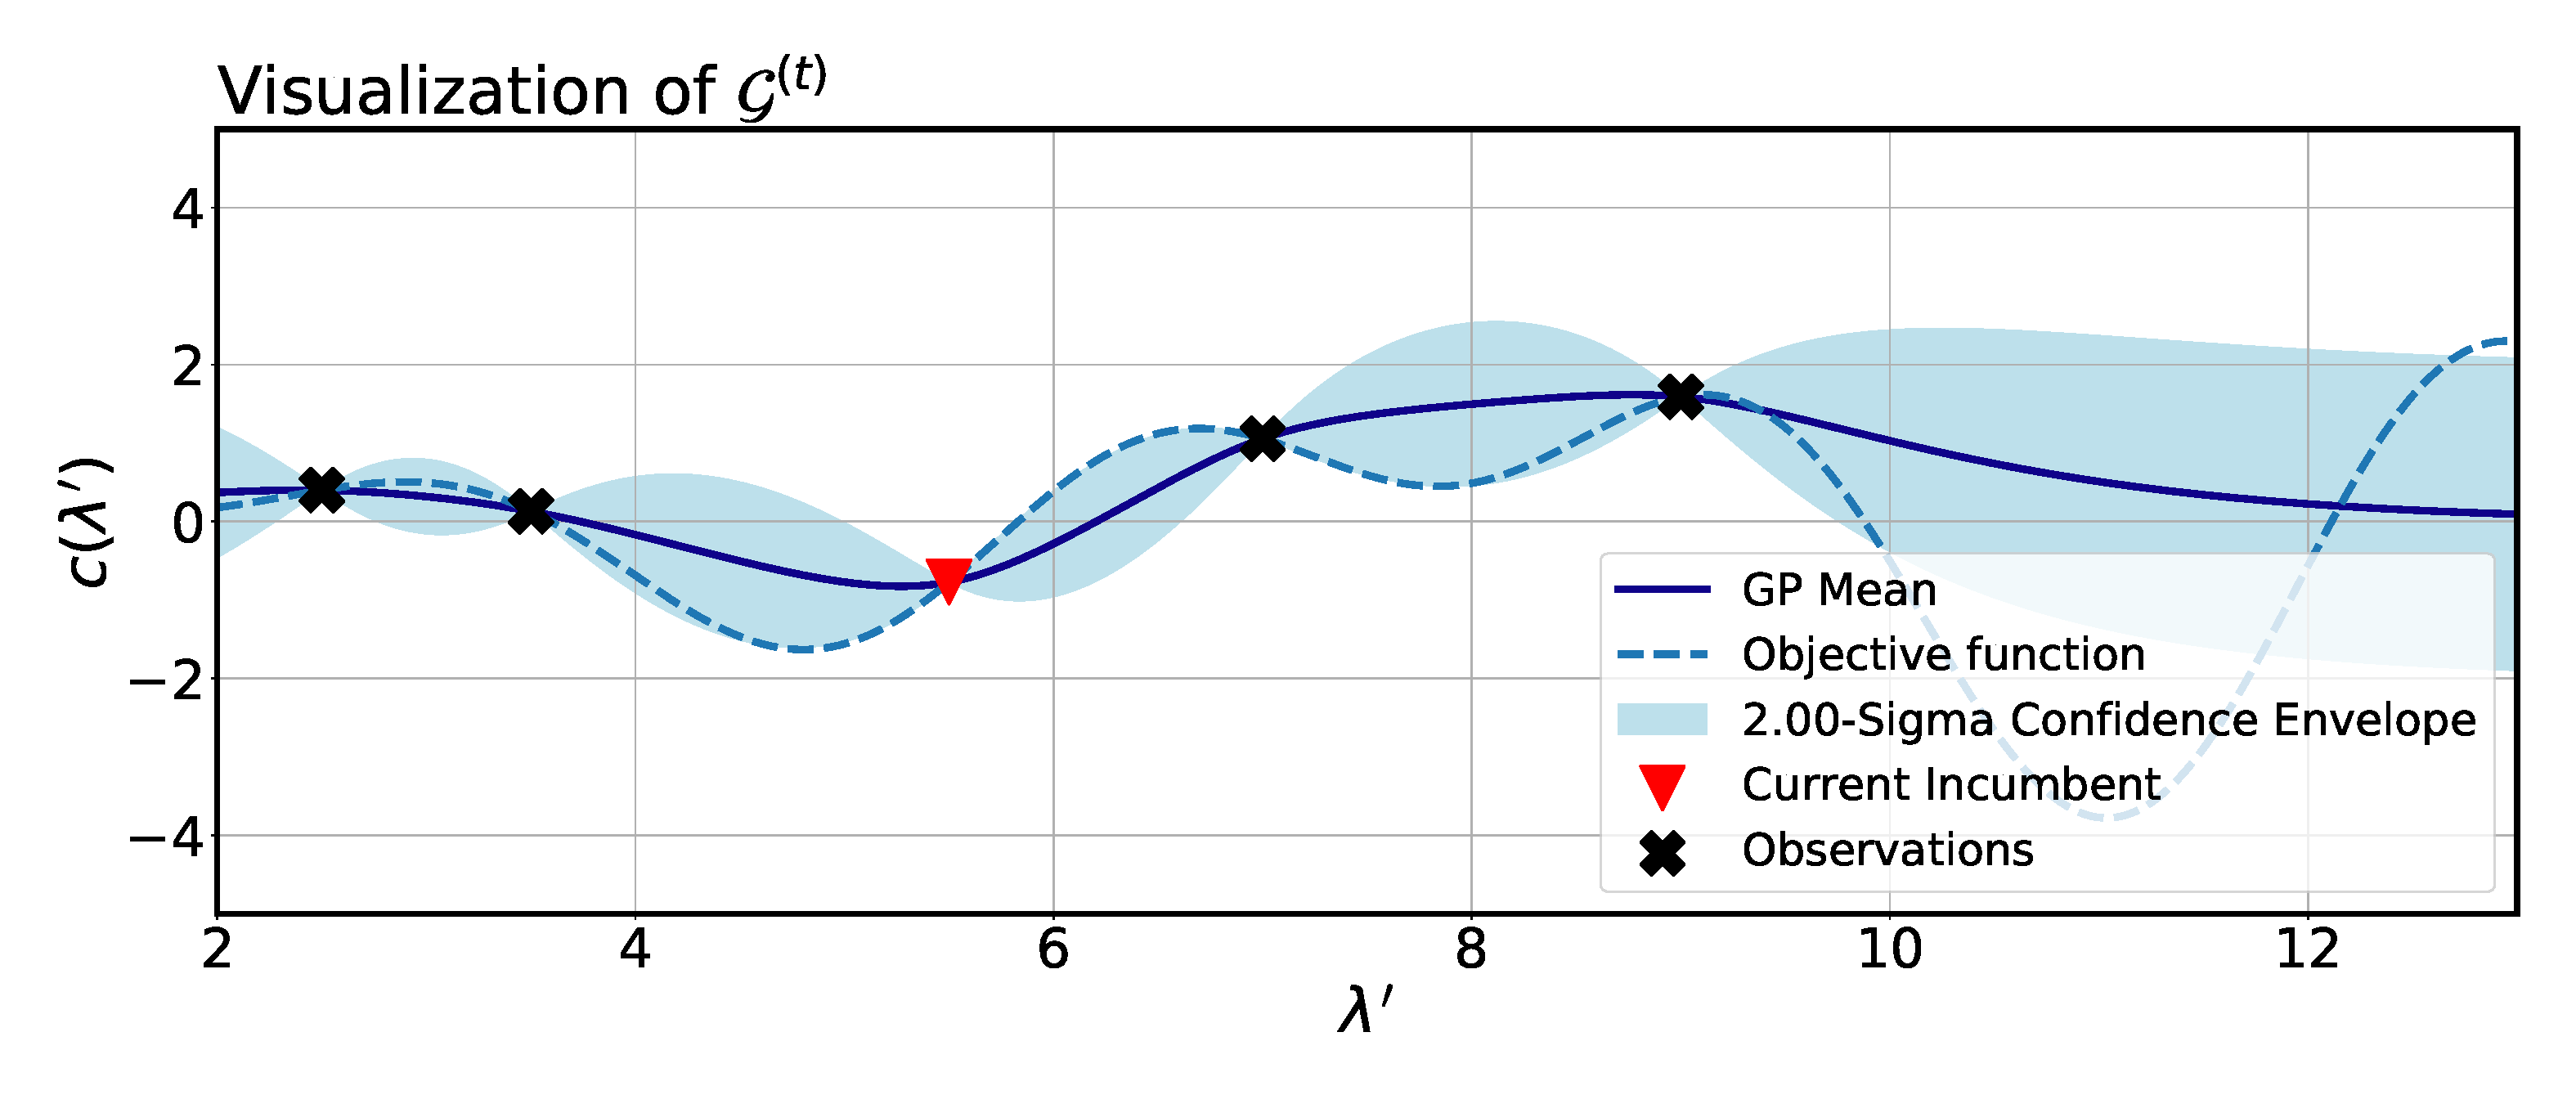
\includegraphics[width=\linewidth, height=0.7\textheight, keepaspectratio=true]{images/acq_func_images/ei/ei_2.pdf}};
    \node<.> [below=0.01\belowcaptionskip of img2, align=center]{Current incumbent $\incumbent[\bocount-1]$ and its observed cost $\cost(\incumbent[\bocount-1])$};

    \node<+> (img3) {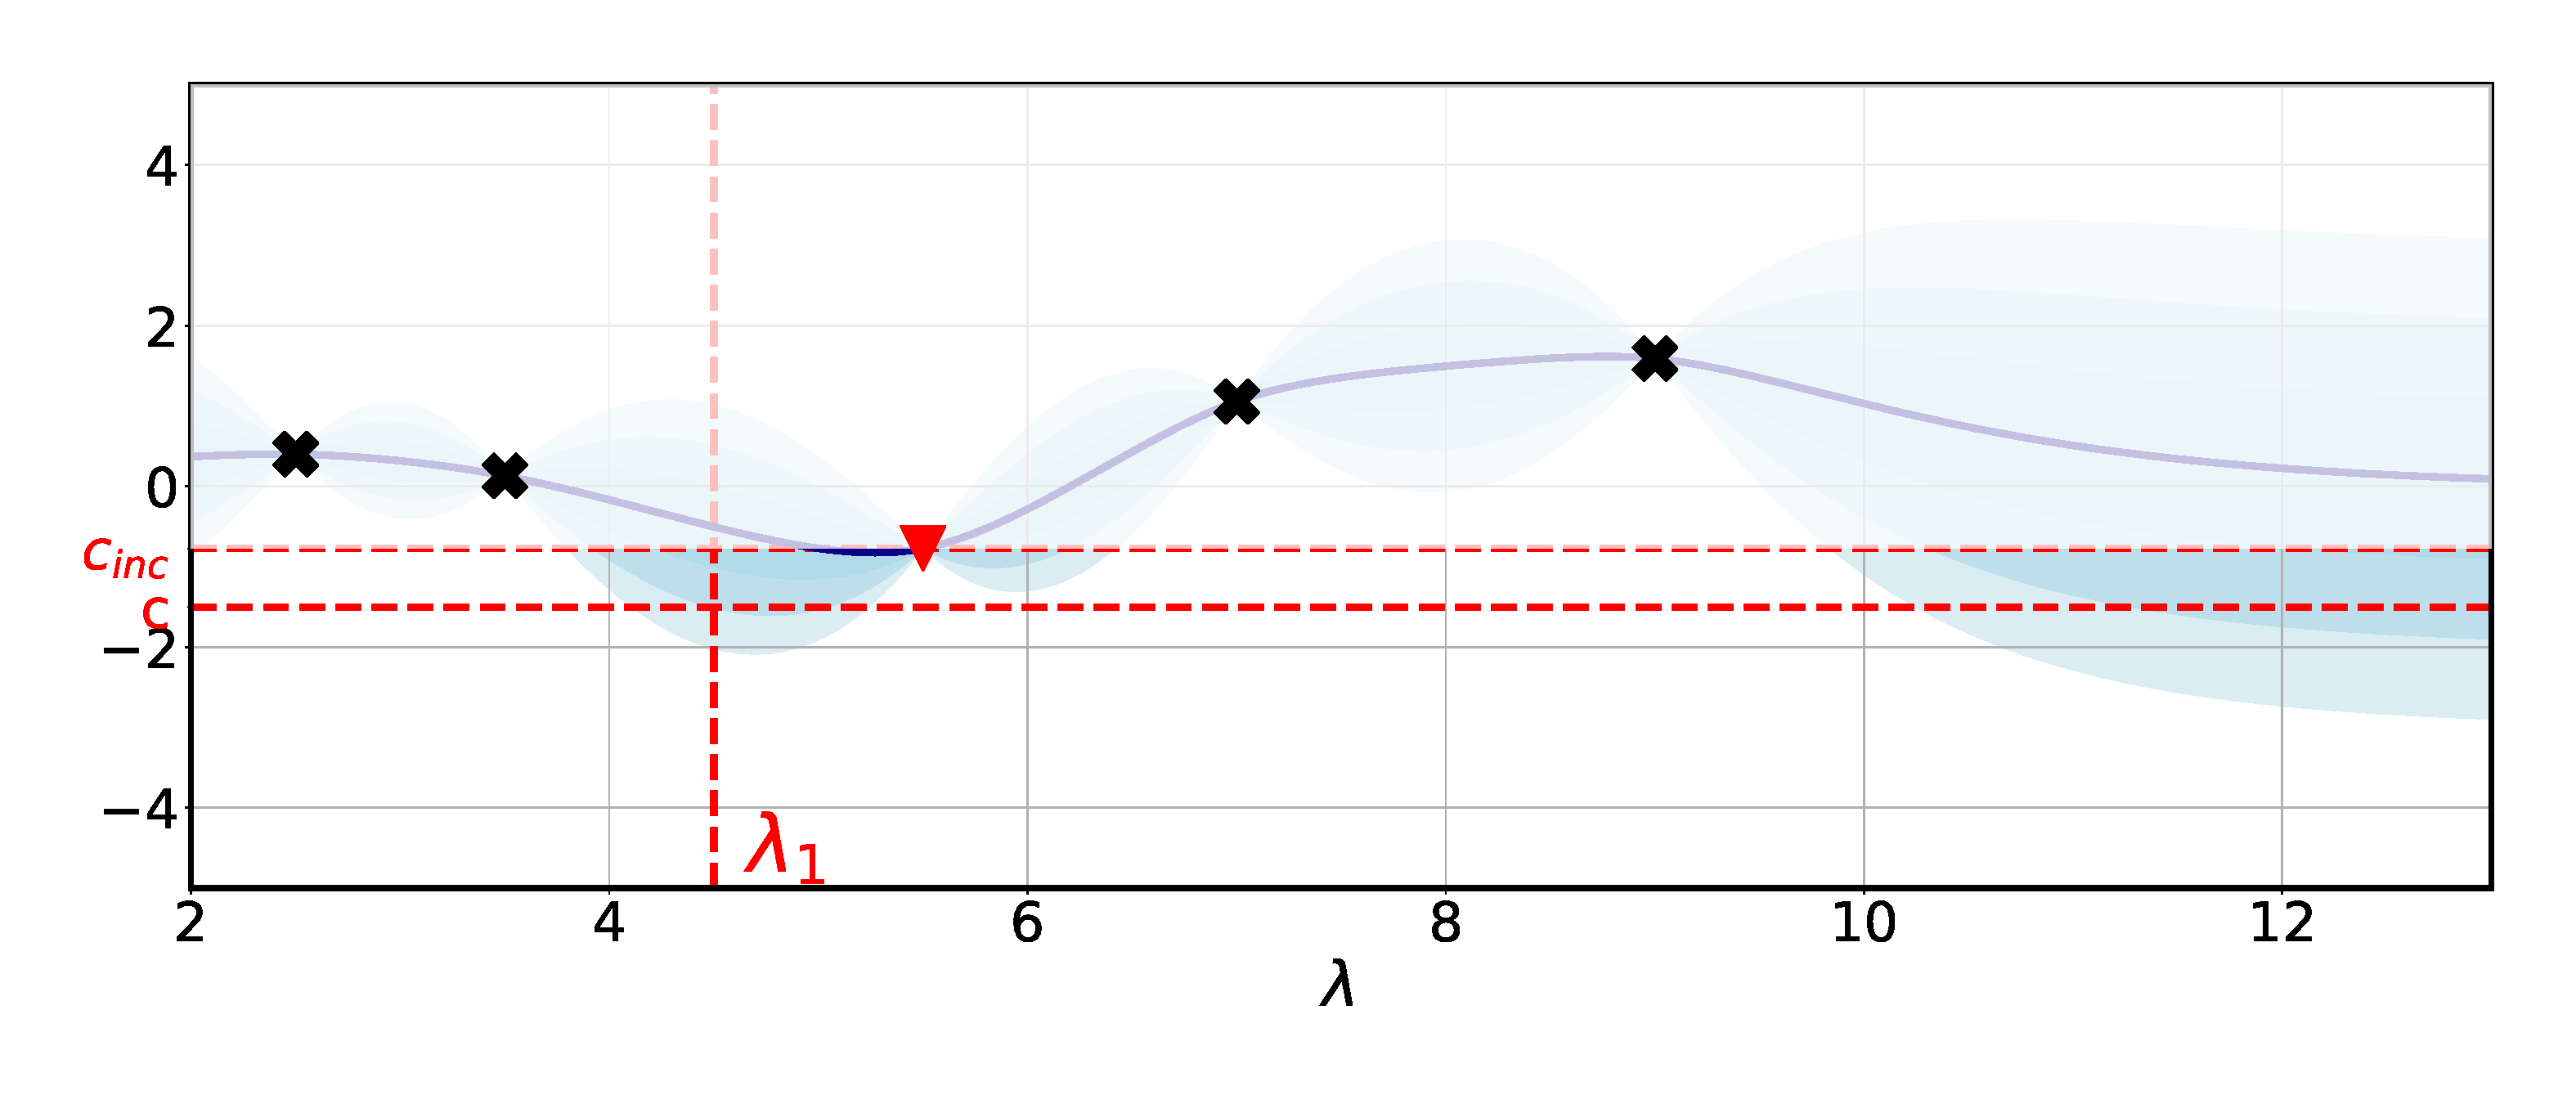
\includegraphics[width=\linewidth, height=0.7\textheight, keepaspectratio=true]{images/acq_func_images/ei/ei_3.pdf}};
    \node<.> [below=0.01\belowcaptionskip of img3, align=center]{Region of Probable Improvement};

    \node<+> (img4) {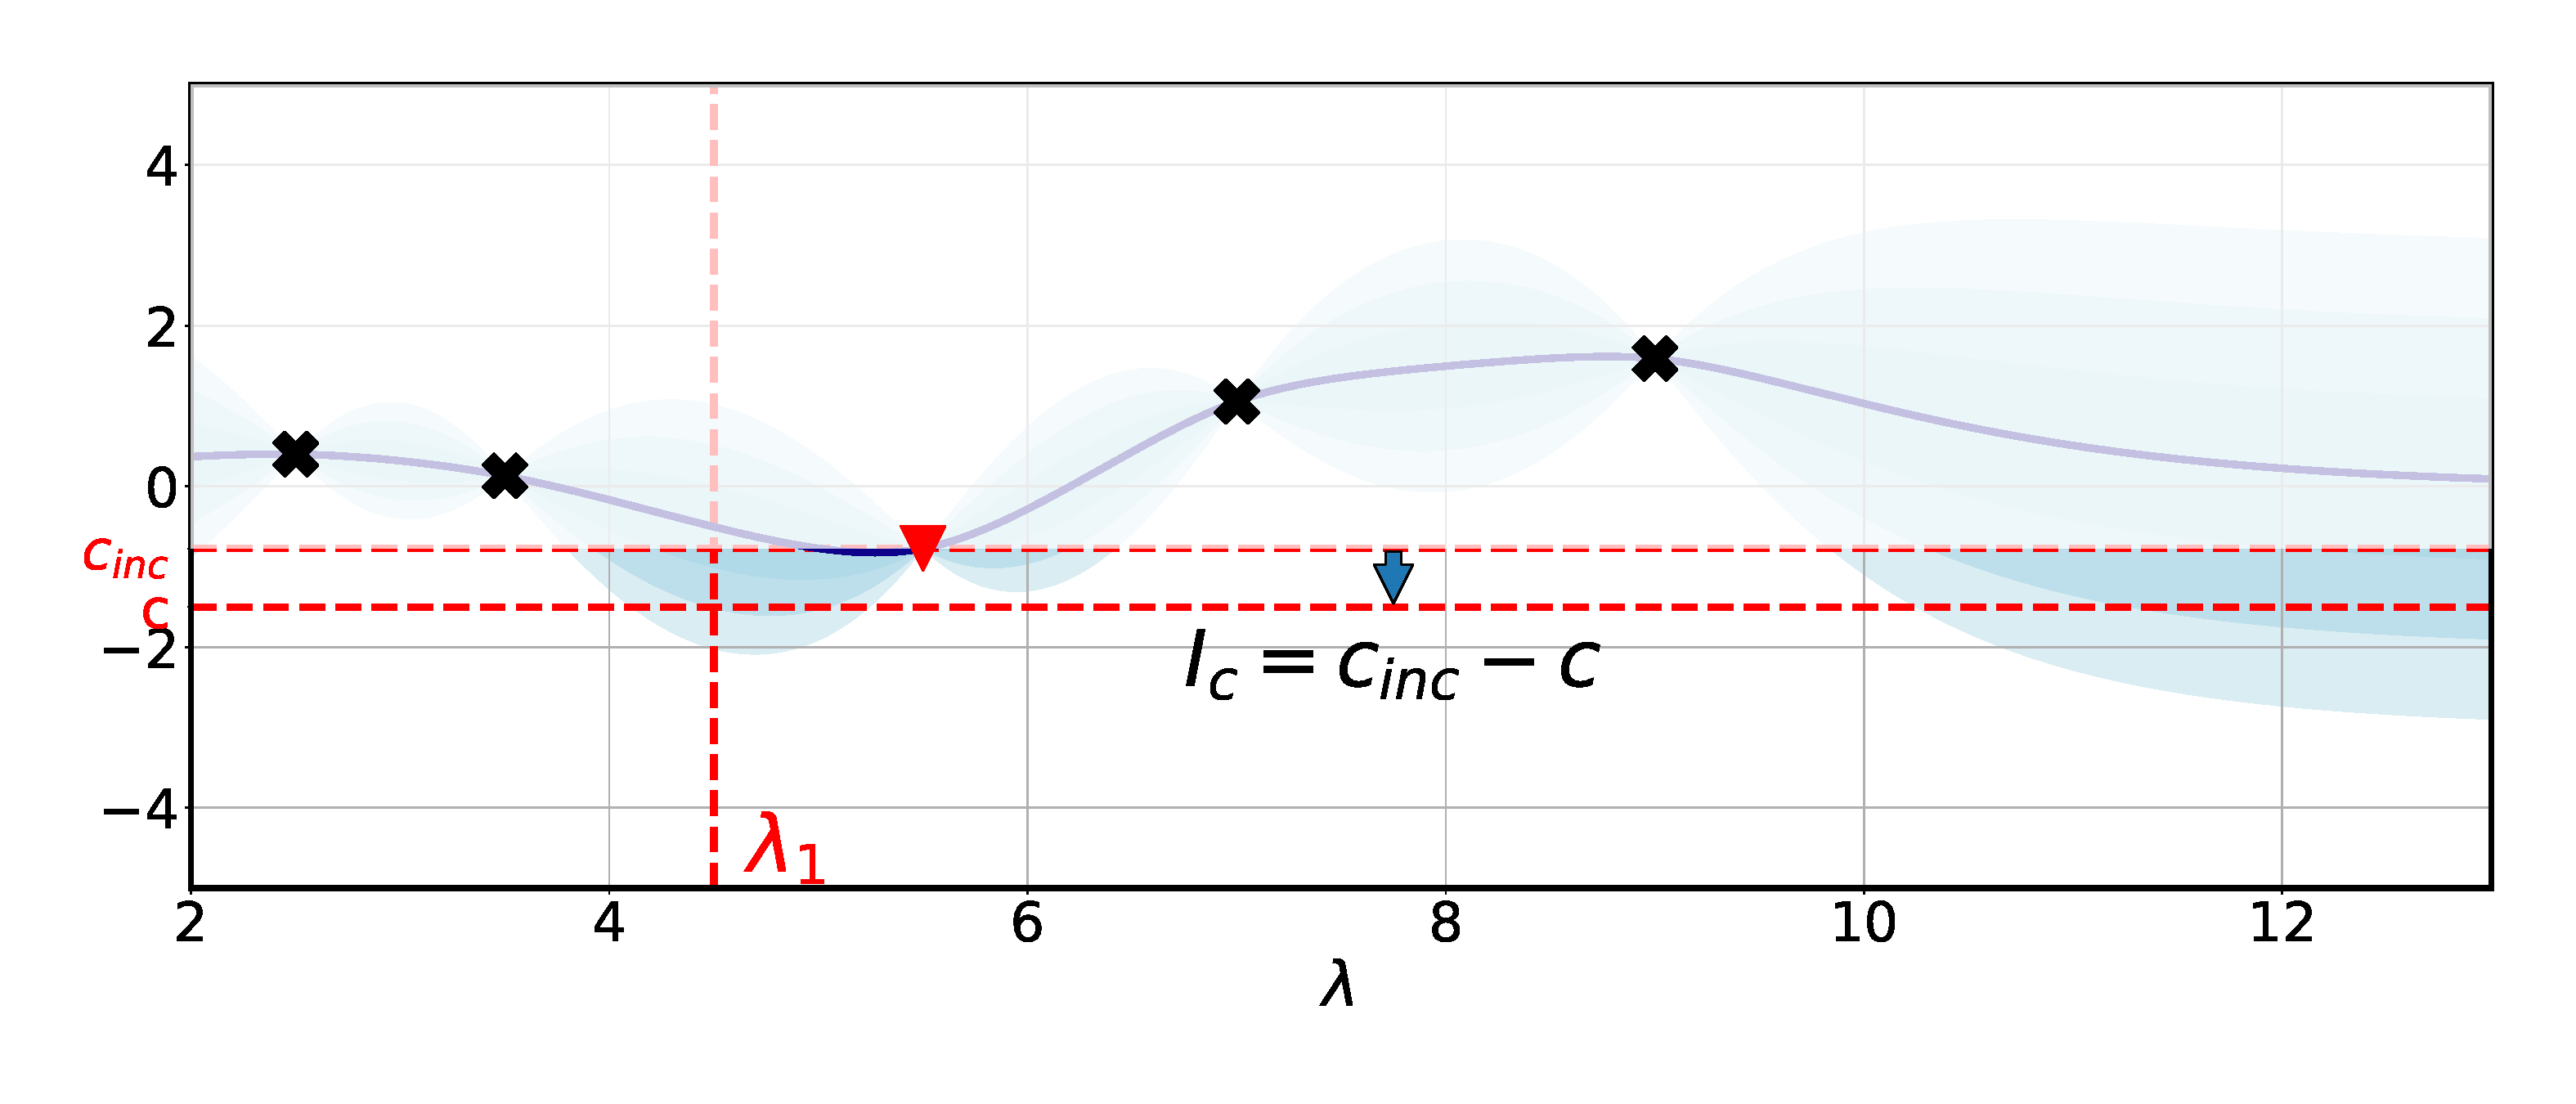
\includegraphics[width=\linewidth, height=0.7\textheight, keepaspectratio=true]{images/acq_func_images/ei/ei_4.pdf}};
    \node<.> [below=0.01\belowcaptionskip of img4, align=center]{Now forget the objective function - it's unknown anyways!};

    \node<+> (img5) {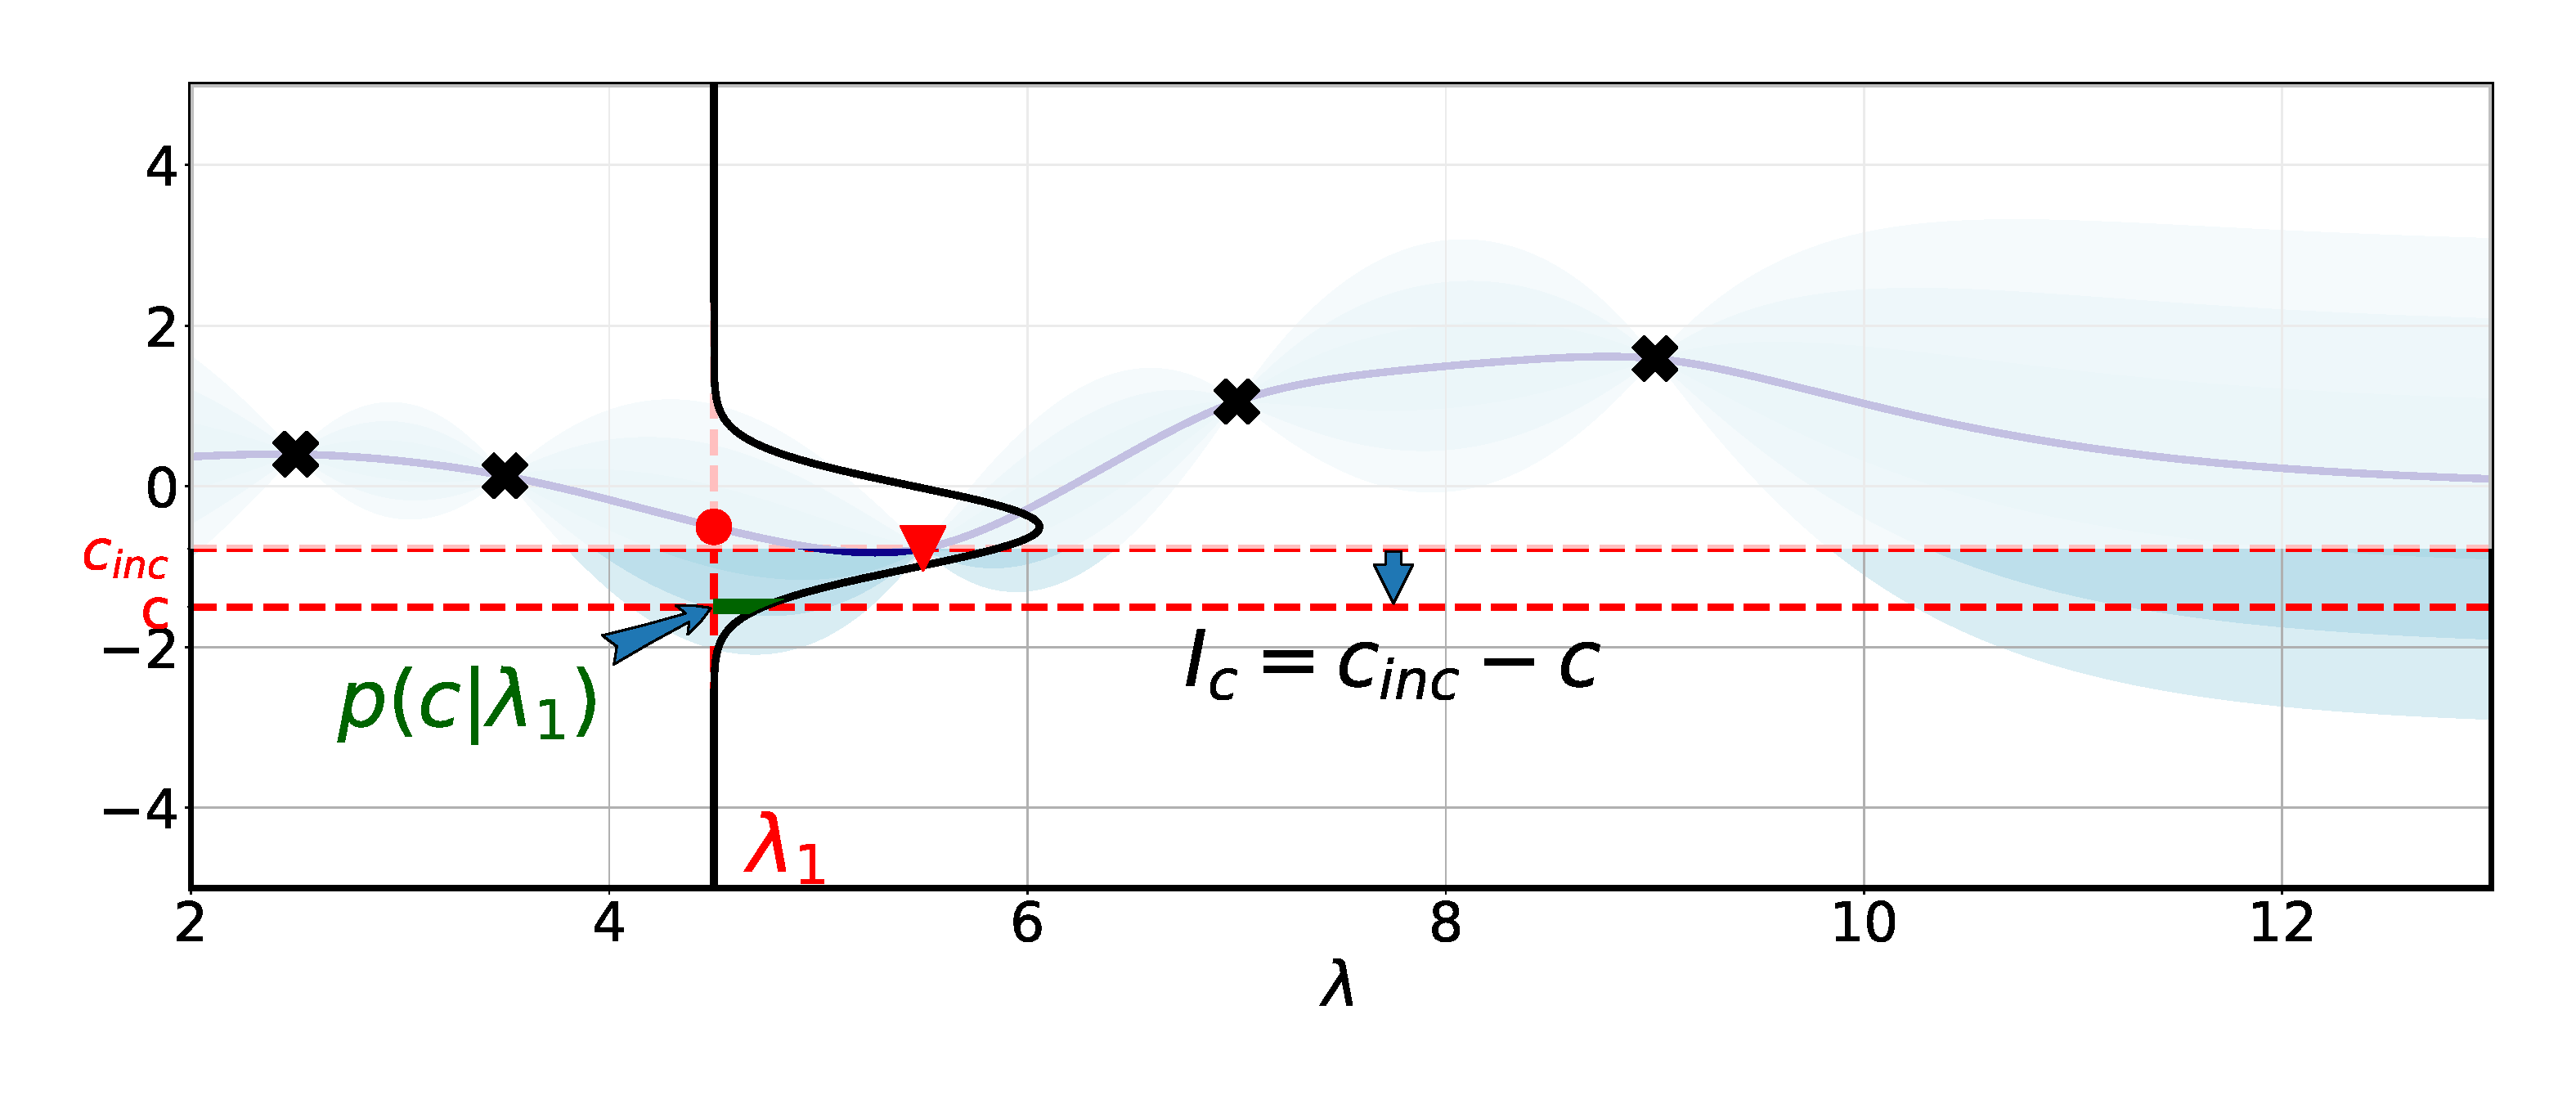
\includegraphics[width=\linewidth, height=0.7\textheight, keepaspectratio=true]{images/acq_func_images/ei/ei_5.pdf}};
    \node<.> [below=0.01\belowcaptionskip of img5, align=center]{Hypothetical \emph{real} cost at a given $\conf$ - unknown in practice without evaluating};

    \node<+> (img6) {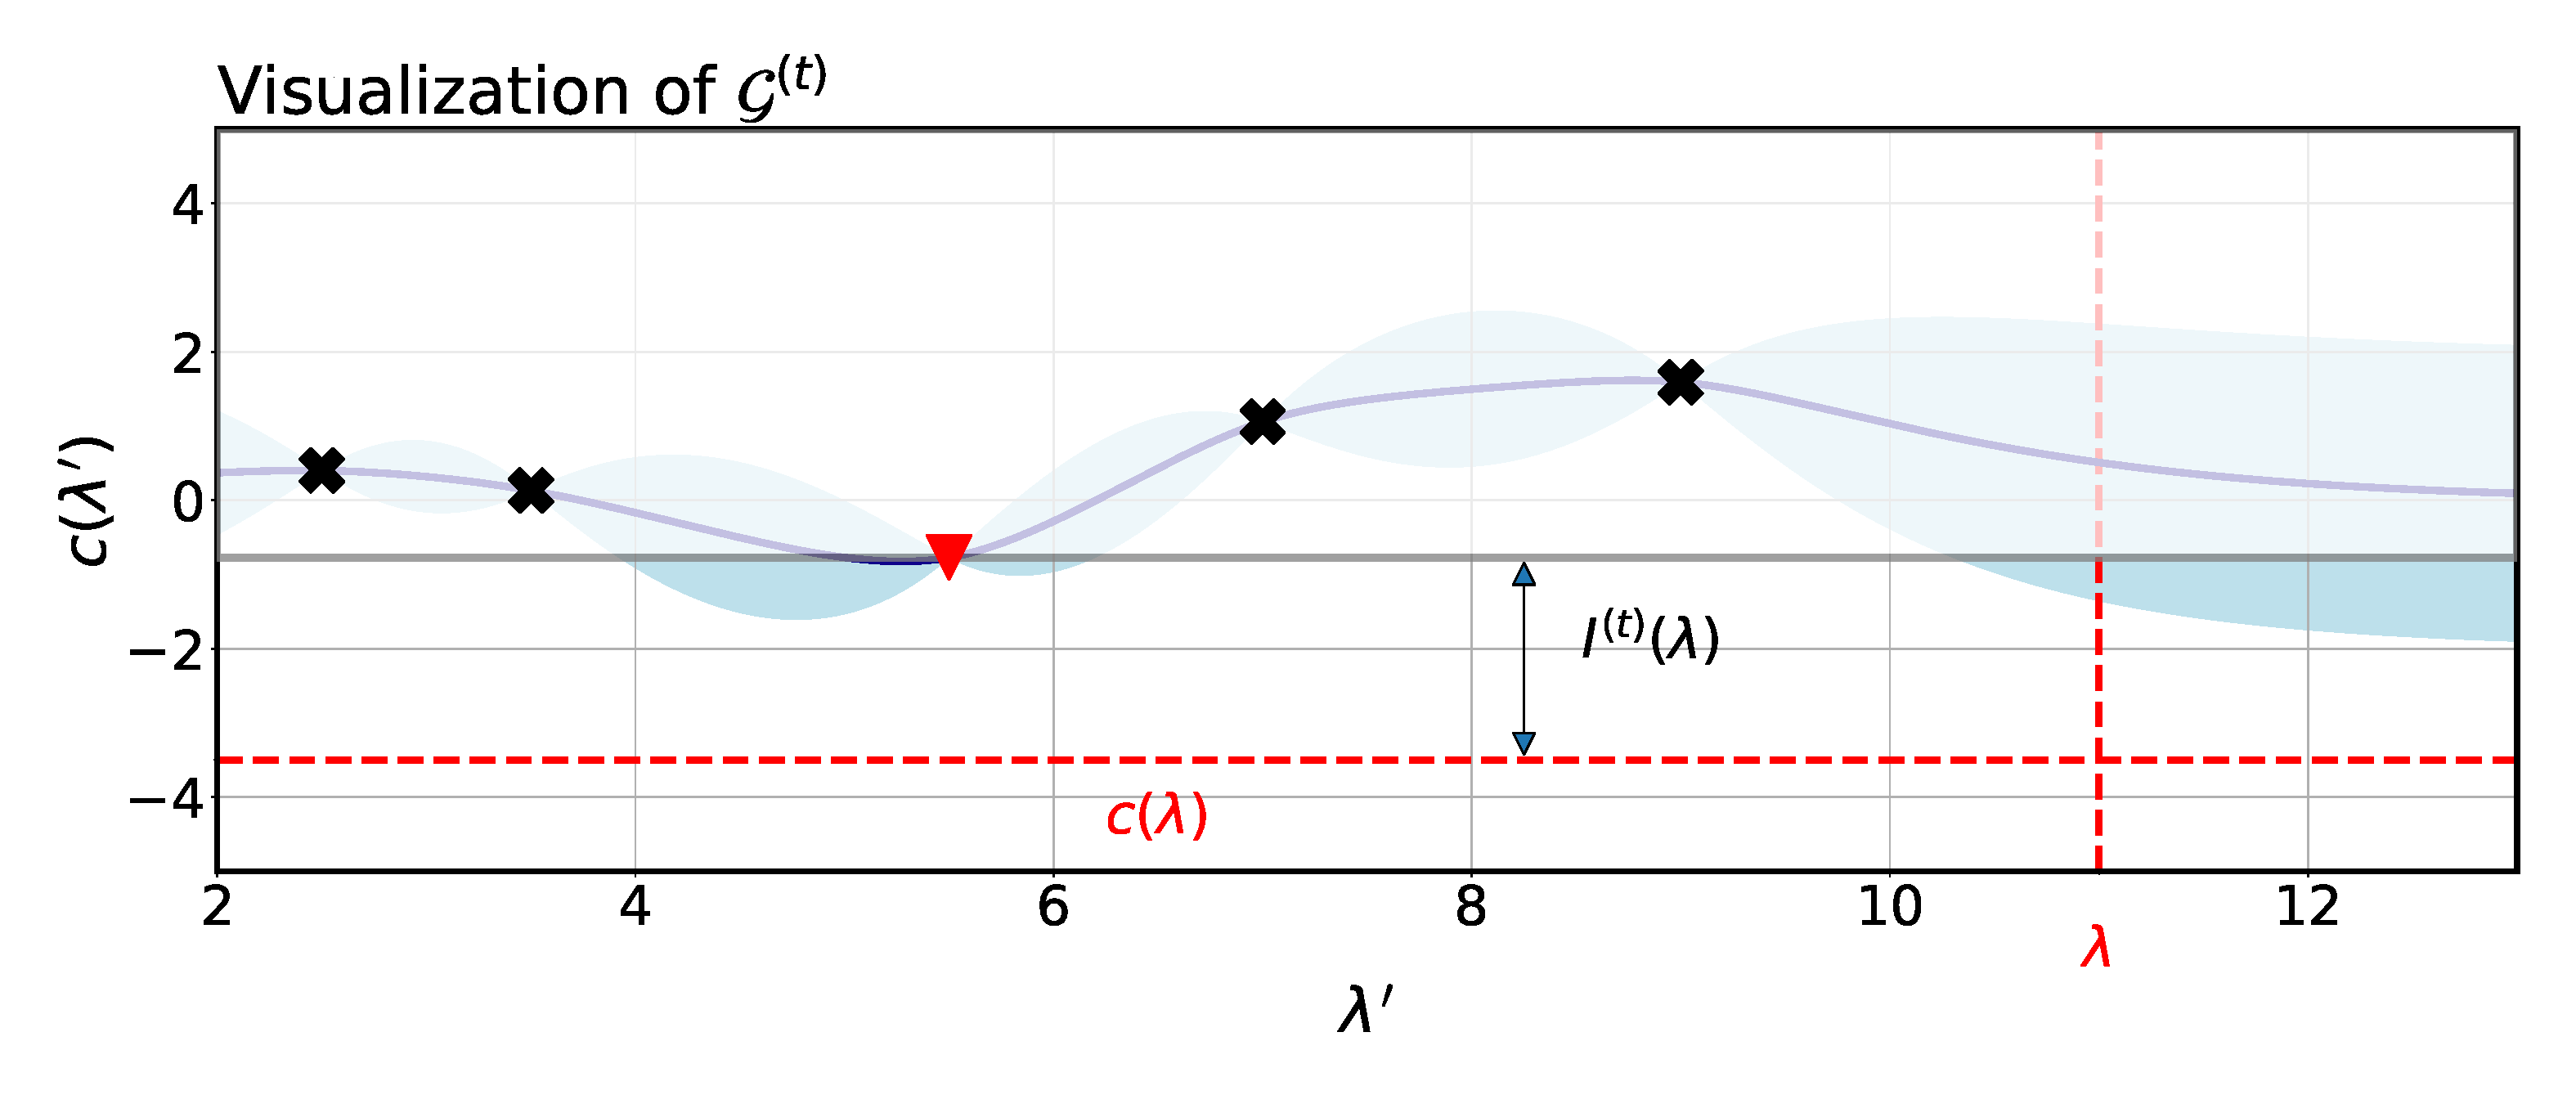
\includegraphics[width=\linewidth, height=0.7\textheight, keepaspectratio=true]{images/acq_func_images/ei/ei_6.pdf}};
    \node<.> [below=-0.01\belowcaptionskip of img6, align=center]{Without performing an actual evaluation, we cannot calculate $\iter{I}(\conf)$};
    
    \node<+> (img7) {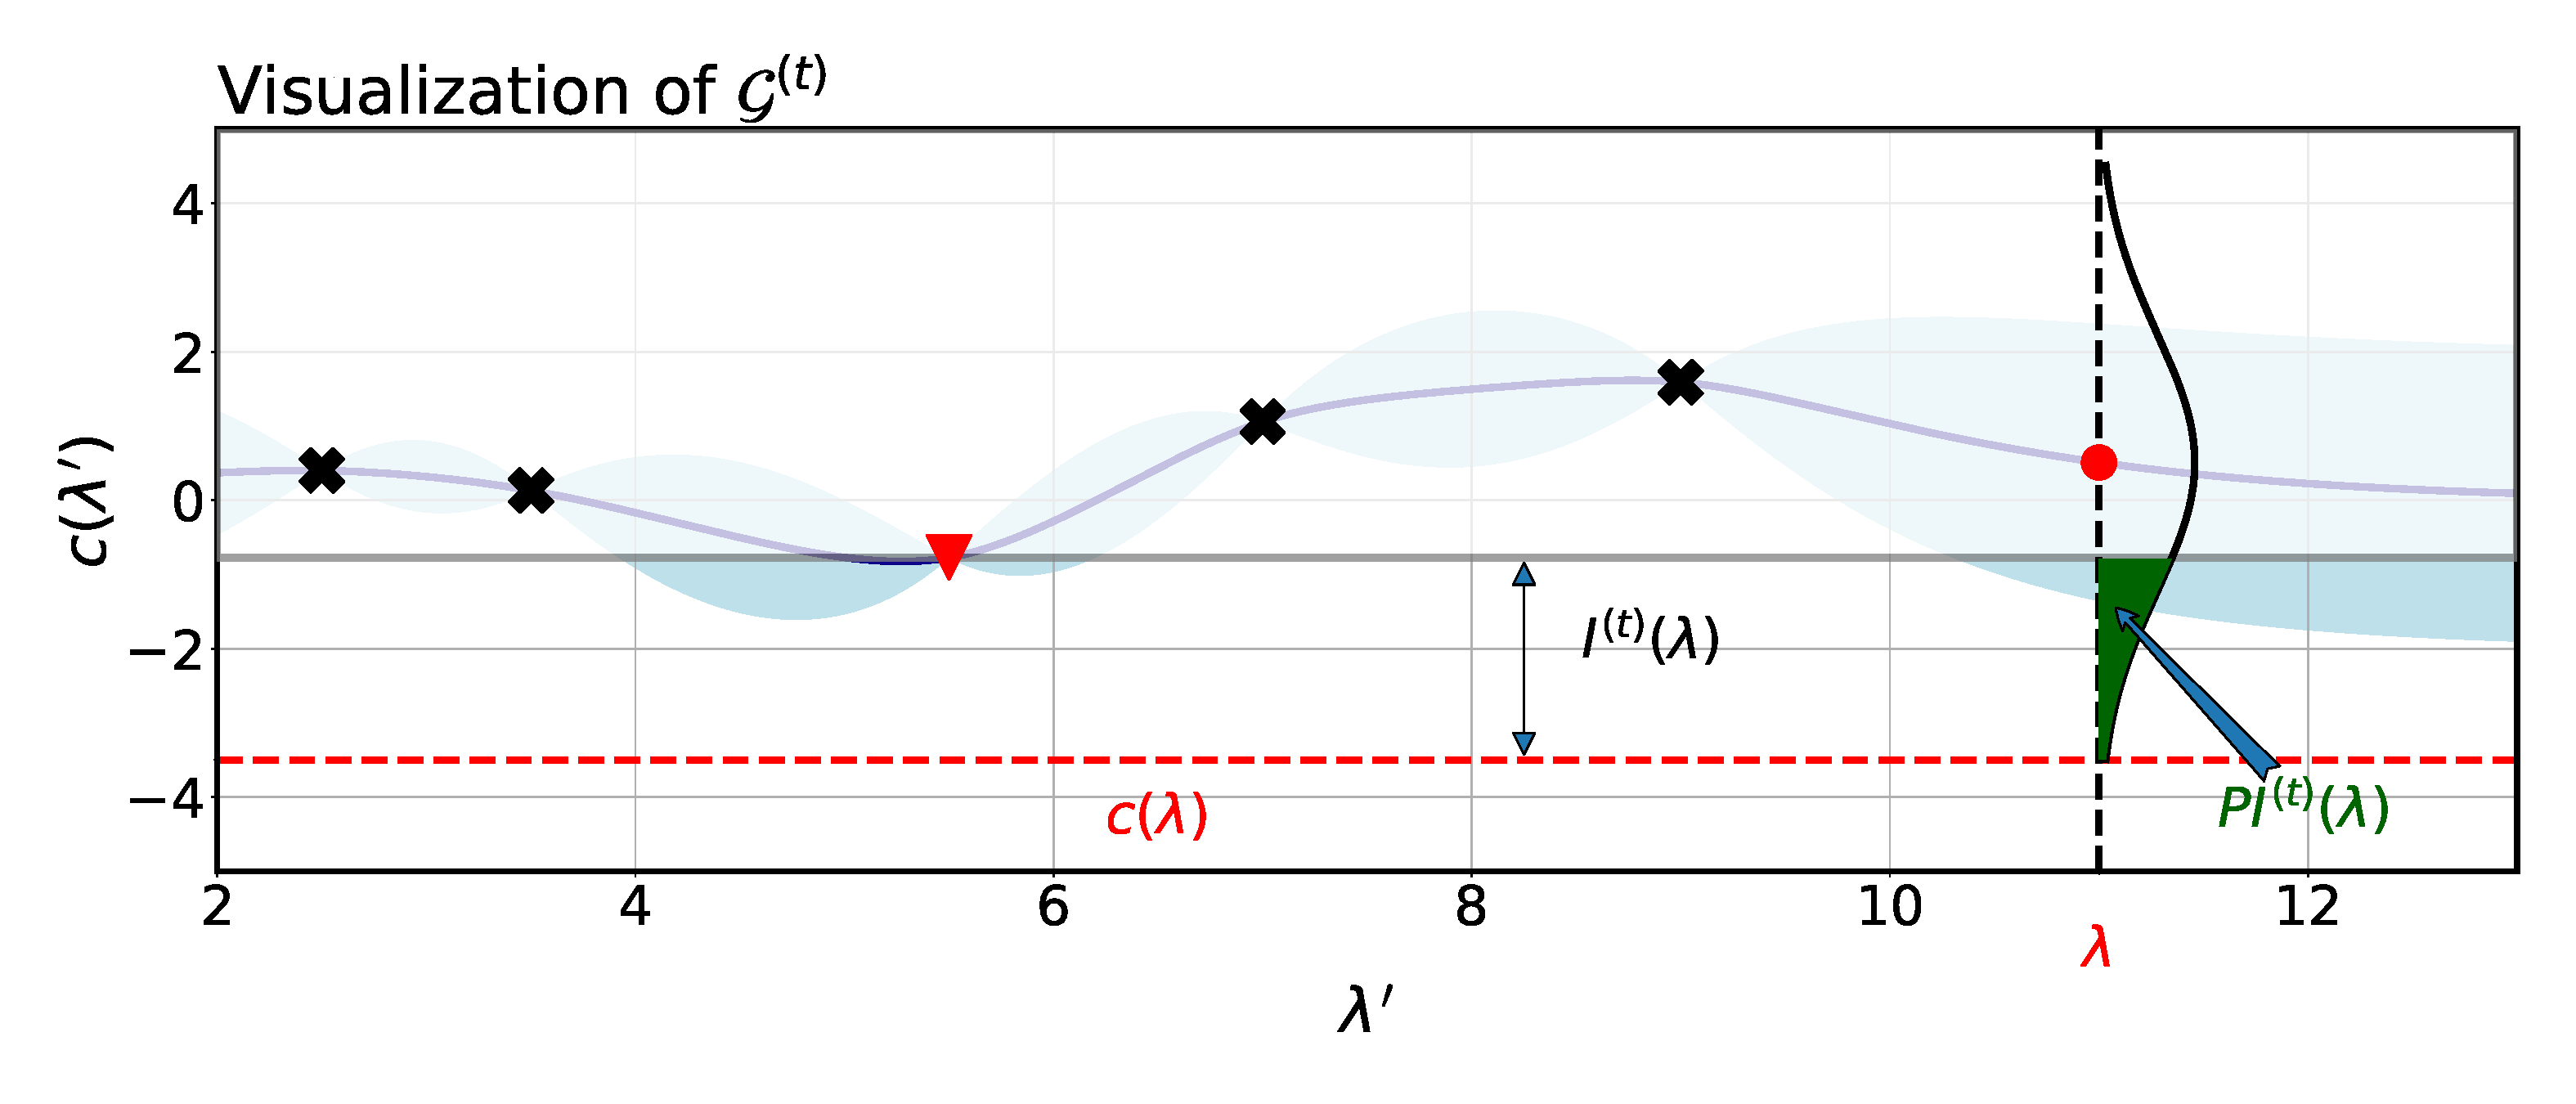
\includegraphics[width=\linewidth, height=0.7\textheight, keepaspectratio=true]{images/acq_func_images/ei/ei_7.pdf}};
    \node<.> [below=0.01\belowcaptionskip of img7, align=center]{Use $P(\conf) = \normaldist (\conf; \iter{\mean}, \iter{(\variance)})$ to calculate $\E[\iter{I}(\conf)]$ instead};
  \end{tikzpicture}
\end{figure}

\end{frame}
%-----------------------------------------------------------------------
\begin{frame}[c]{Computationally Cheap Acquisition Functions - EI}
\framesubtitle{Expected Improvement - Choosing a candidate}
\comment{Verify if formulae agree with minimizing the surrogate.}
    \begin{itemize}\abovedisplayskip=0pt\belowdisplayskip=-0.5em
        \item[] We first define one-step improvement over the current incumbent, as
        \smallskip
        \[
            \iter{I}(\conf) = \max(0, \cost(\incumbent[\bocount-1]) - \cost(\conf)), \quad\incumbent[\bocount-1]\in\argmin_{\conf'\in\iter[\bocount-1]{\dataset}}\obs[\conf']\in\iter[\bocount-1]{\dataset}
        \]
        \comment{This is probably a great time to point out, once again, that because I is defined in terms of the actual cost function, we cannot directly compute it.}
        \pause
        \medskip
        \item[] Expected Improvement is then defined as
        \begin{align*}
            \iter{\acq}_{EI}(\conf) &= \E[\iter{I}(\conf)]\\
            &= \int_{\iter{I}=0}^{\iter{I}=\infty}\iter{I} P(\iter{I})d\iter{I}
        \end{align*}
        \pause
        \medskip
        \item[]Since the posterior distribution of the surrogate is a Gaussian, it can be shown that the distribution on $\iter{I}(\conf)$ is also a Gaussian, defined as
        \[
            P(\iter{I}) =
                \dfrac{1}{\sqrt{2\pi}\iter{\stddev}(\conf)}\exp{-\dfrac{{(\cost(\incumbent[\bocount-1])-\iter{\mean}(\conf)-\iter{I})}^2}{2\iter{\left(\variance\right)}(\conf)}
            }
        \]
        \comment{Maybe emphasize that this is actually how and where the dependence on the actual cost function is replaced with a dependence on the surrogate.}
    \end{itemize}
\end{frame}
%-----------------------------------------------------------------------
% \begin{frame}[c]{Computationally Cheap Acquisition Functions - EI}
% \framesubtitle{Expected Improvement - Choosing a candidate}
%     \begin{align*}
%         \action<+->{\iter{\acq}_{EI}(\conf) &= \int_{\iter{I}=0}^{\iter{I}=\infty}\iter{I} \dfrac{1}{\sqrt{2\pi}\iter{\stddev}(\conf)}\exp{-\dfrac{{(\cost(\incumbent[\bocount-1])-\iter{\mean}(\conf)-\iter{I})}^2}{2\iter{\left(\variance\right)}(\conf)}}d\iter{I}\\}
%         \action<+->{&= 
%             \begin{cases}
%                 (\cost(\incumbent) - \iter{\mean}(\conf) - \xi)\cdf(Z) + \iter{\stddev}(\conf) \pdf(Z), & \text{if }\iter{\stddev}(\conf) > 0 \\
%                 0 & \text{if }\iter{\stddev}(\conf) = 0
%             \end{cases}\\}
%         \action<+->{\intertext{where }Z} \action<.->{&=\dfrac{\cost(\incumbent) - \iter{\mean}(\conf) - \xi}{\iter{\stddev}(\conf)}}
%     \action<+->{\Aboxed{\bonextsample \in \argmax_{\conf\in\pcs}(\iter{\acq}_{EI}(\conf))}}
%     \end{align*}
% %    \comment{Source: Tutorial by Brochu et al.: https://arxiv.org/pdf/1012.2599.pdf }
% \end{frame}
%-----------------------------------------------------------------------
\begin{frame}[c]{Computationally Cheap Acquisition Functions - EI}
\framesubtitle{Expected Improvement - Choosing a candidate}
    \begin{align*}
        \action<+->{\iter{\acq}_{EI}(\conf) &= \int_{\iter{I}=0}^{\iter{I}=\infty}\iter{I} \dfrac{1}{\sqrt{2\pi}\iter{\stddev}(\conf)}\exp{-\dfrac{{(\cost(\incumbent[\bocount-1])-\iter{\mean}(\conf)-\iter{I})}^2}{2\iter{\left(\variance\right)}(\conf)}}d\iter{I}\\}
        \action<+->{&= 
            \begin{cases}
                \iter{\stddev}(\conf)[Z\cdf(Z) + \pdf(Z)], & \text{if }\iter{\stddev}(\conf) > 0 \\
                0 & \text{if }\iter{\stddev}(\conf) = 0
            \end{cases}\\
            \intertext{where }Z &=\dfrac{\cost(\incumbent[\bocount-1]) - \iter{\mean}(\conf) - \xi}{\iter{\stddev}(\conf)}}
            \comment{I believe I needed to switch the signs of $\cost(\cdot)$ and $\mean(\cdot)$ as compared to the reference paper in order to accommodate for our convention of minimization/maximization. Please cross-check!}
    \action<+->{\Aboxed{\text{Choose}\,\bonextsample \in \argmax_{\conf\in\pcs}(\iter{\acq}_{EI}(\conf))}}
    \end{align*}
%    \comment{Source: Tutorial by Brochu et al.: https://arxiv.org/pdf/1012.2599.pdf }
\end{frame}
%-----------------------------------------------------------------------
\begin{frame}[t]{Computationally Cheap Acquisition Functions - LCB/UCB}
\framesubtitle{Confidence Bounds - Concept}

\begin{figure}
  \centering
  \begin{tikzpicture}
    \node<+> (img1) {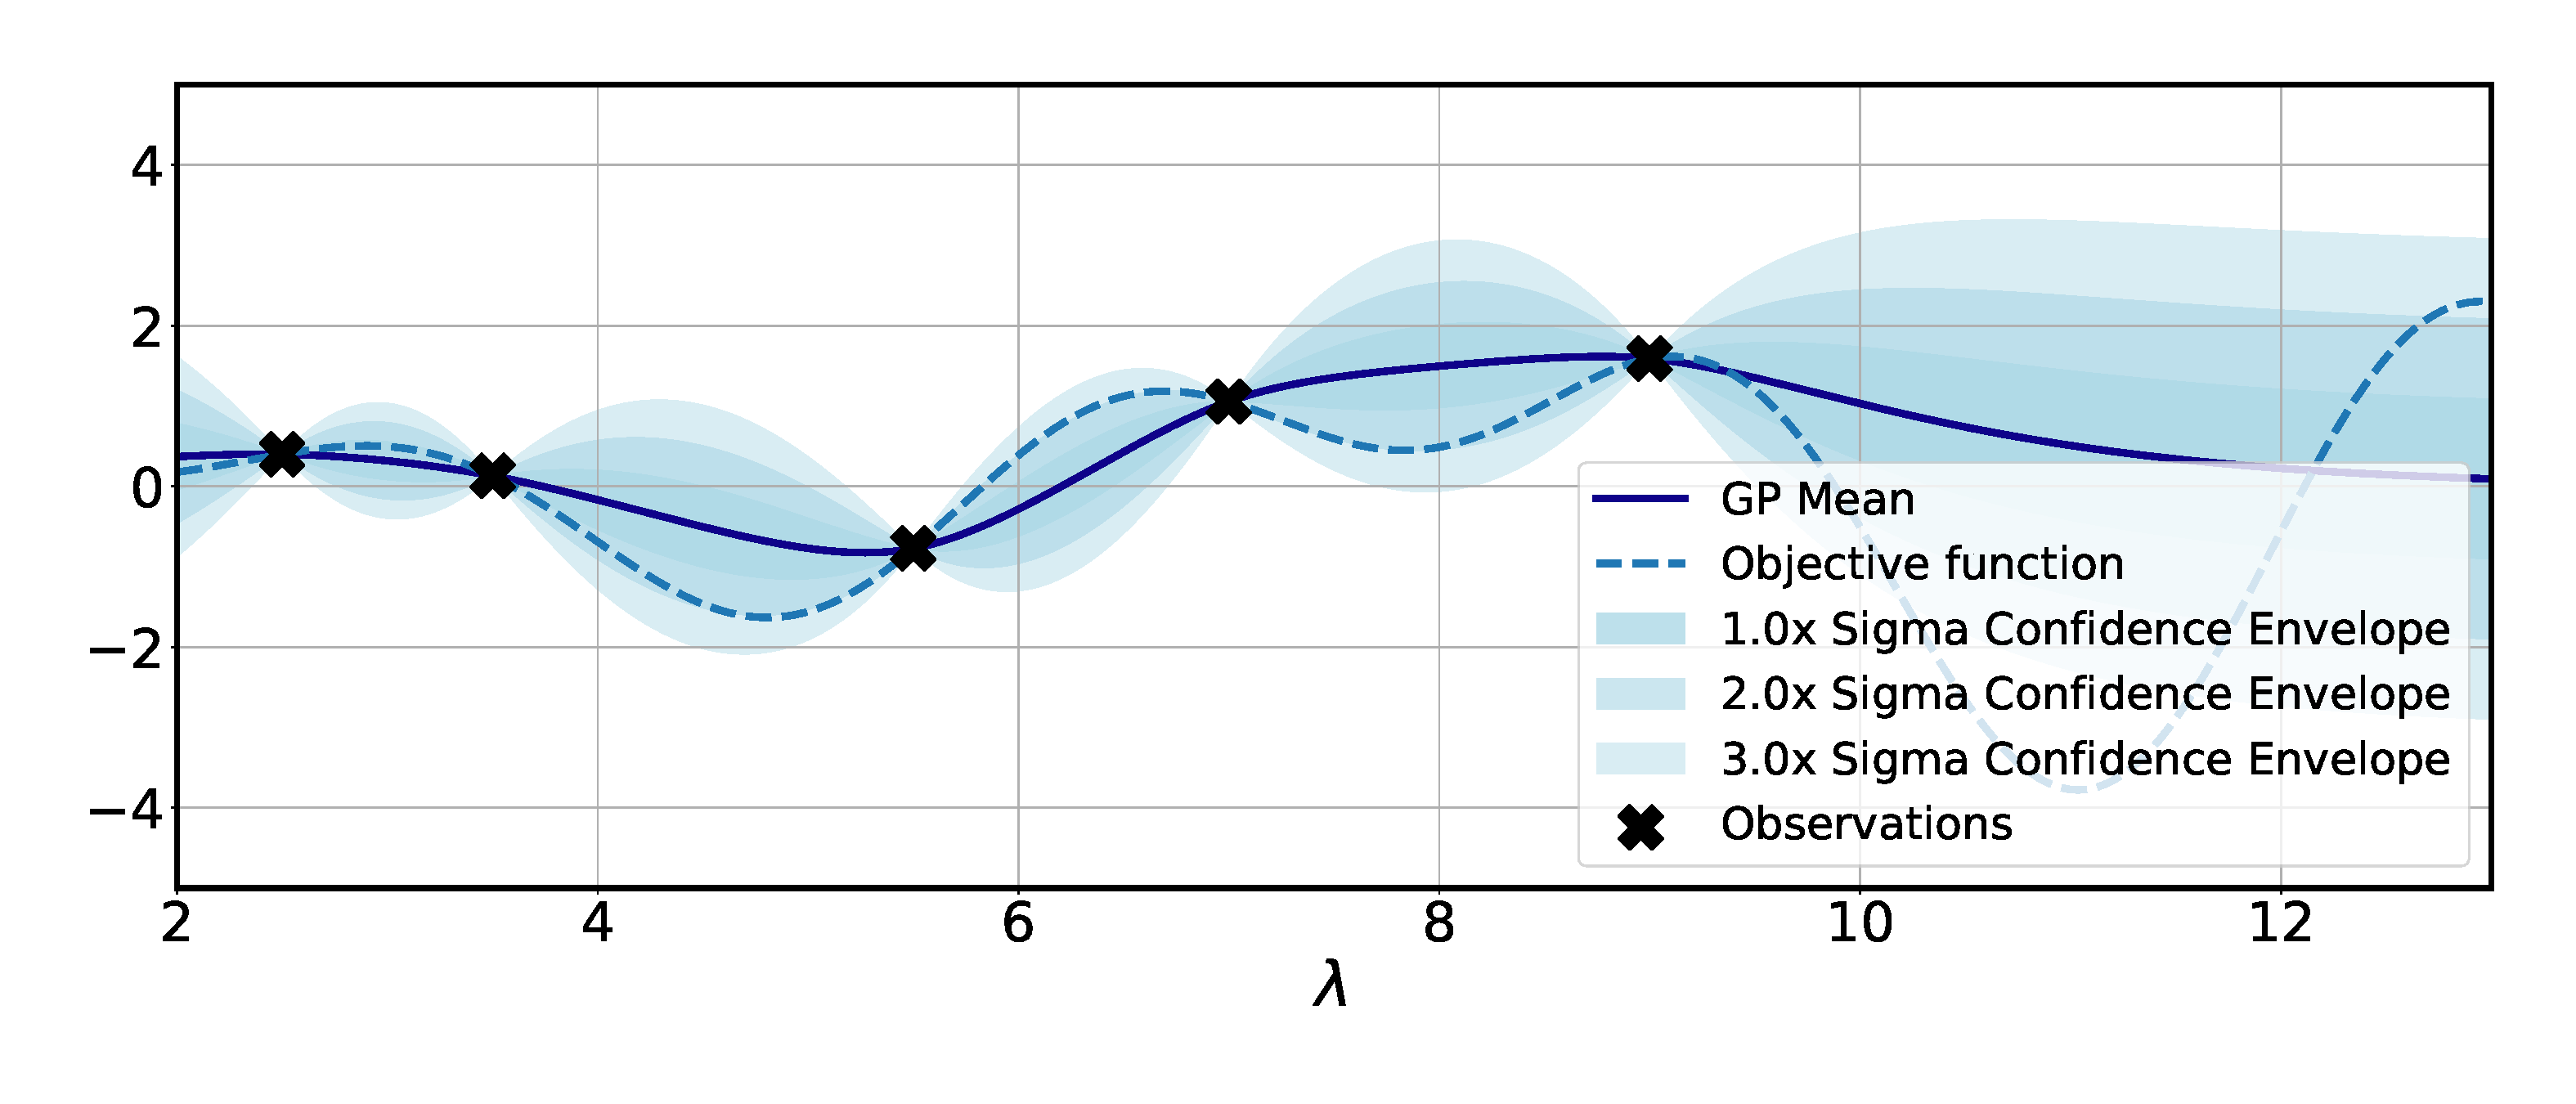
\includegraphics[width=\linewidth, height=0.7\textheight, keepaspectratio=true]{images/acq_func_images/lcb/lcb_1.pdf}};
    \node<.> [below=0.01\belowcaptionskip of img1, align=center]{Confidence Bound, $\mean(\conf)\pm\alpha\stddev(\conf)$};
    \node<+> (img2) {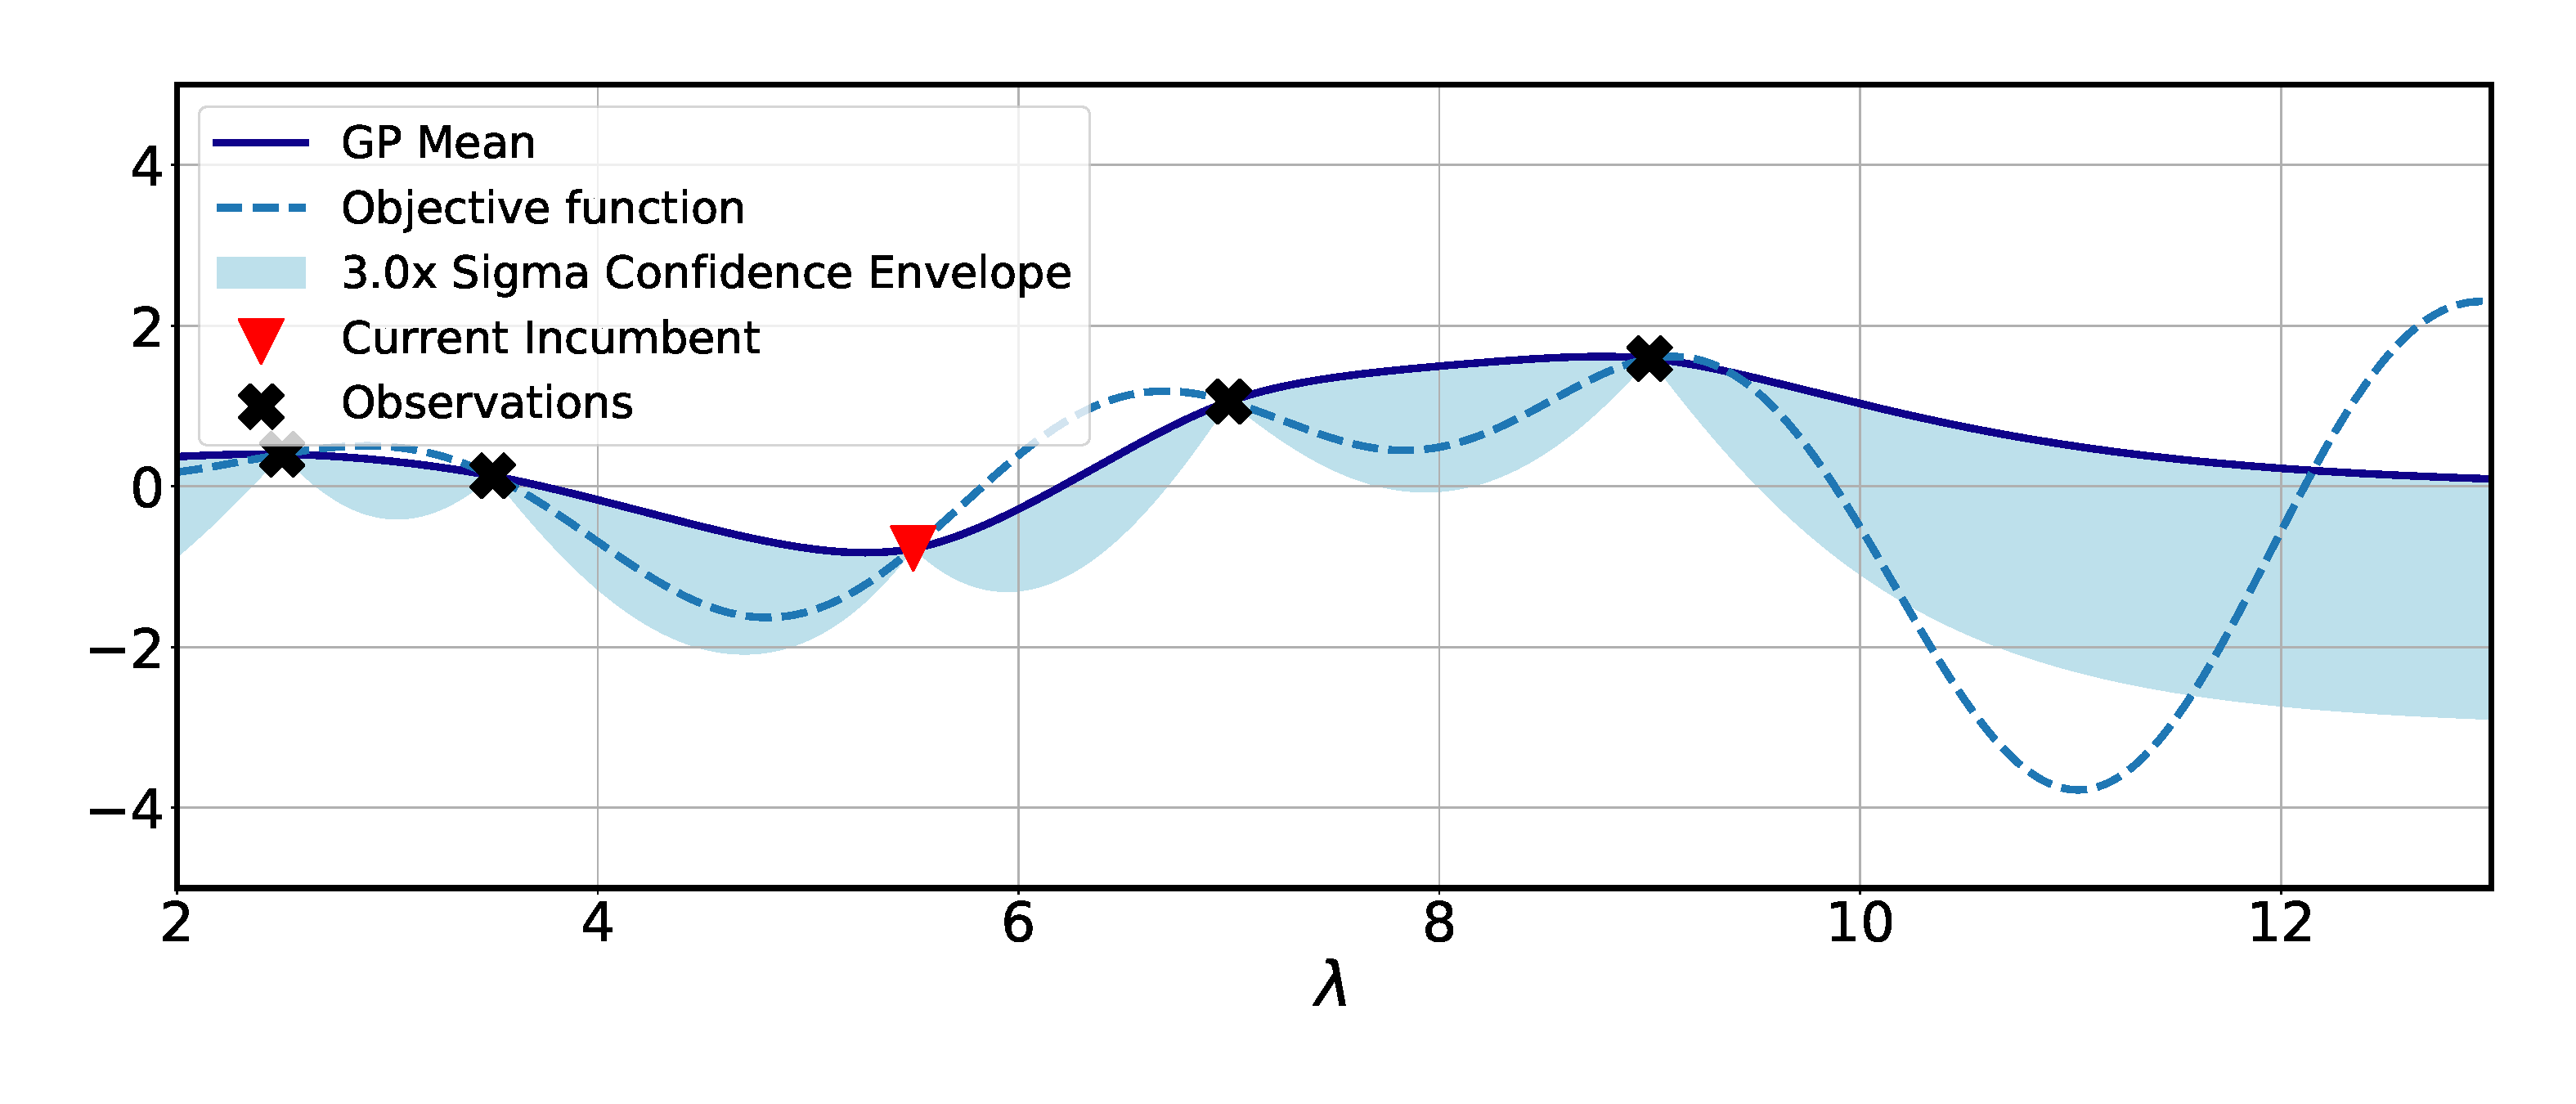
\includegraphics[width=\linewidth, height=0.7\textheight, keepaspectratio=true]{images/acq_func_images/lcb/lcb_2.pdf}};
    \node<.> [below=0.01\belowcaptionskip of img2, align=center]{Lower Confidence Bound, $\mean(\conf)-\alpha\stddev(\conf)$.};
    \node<+> (img3) {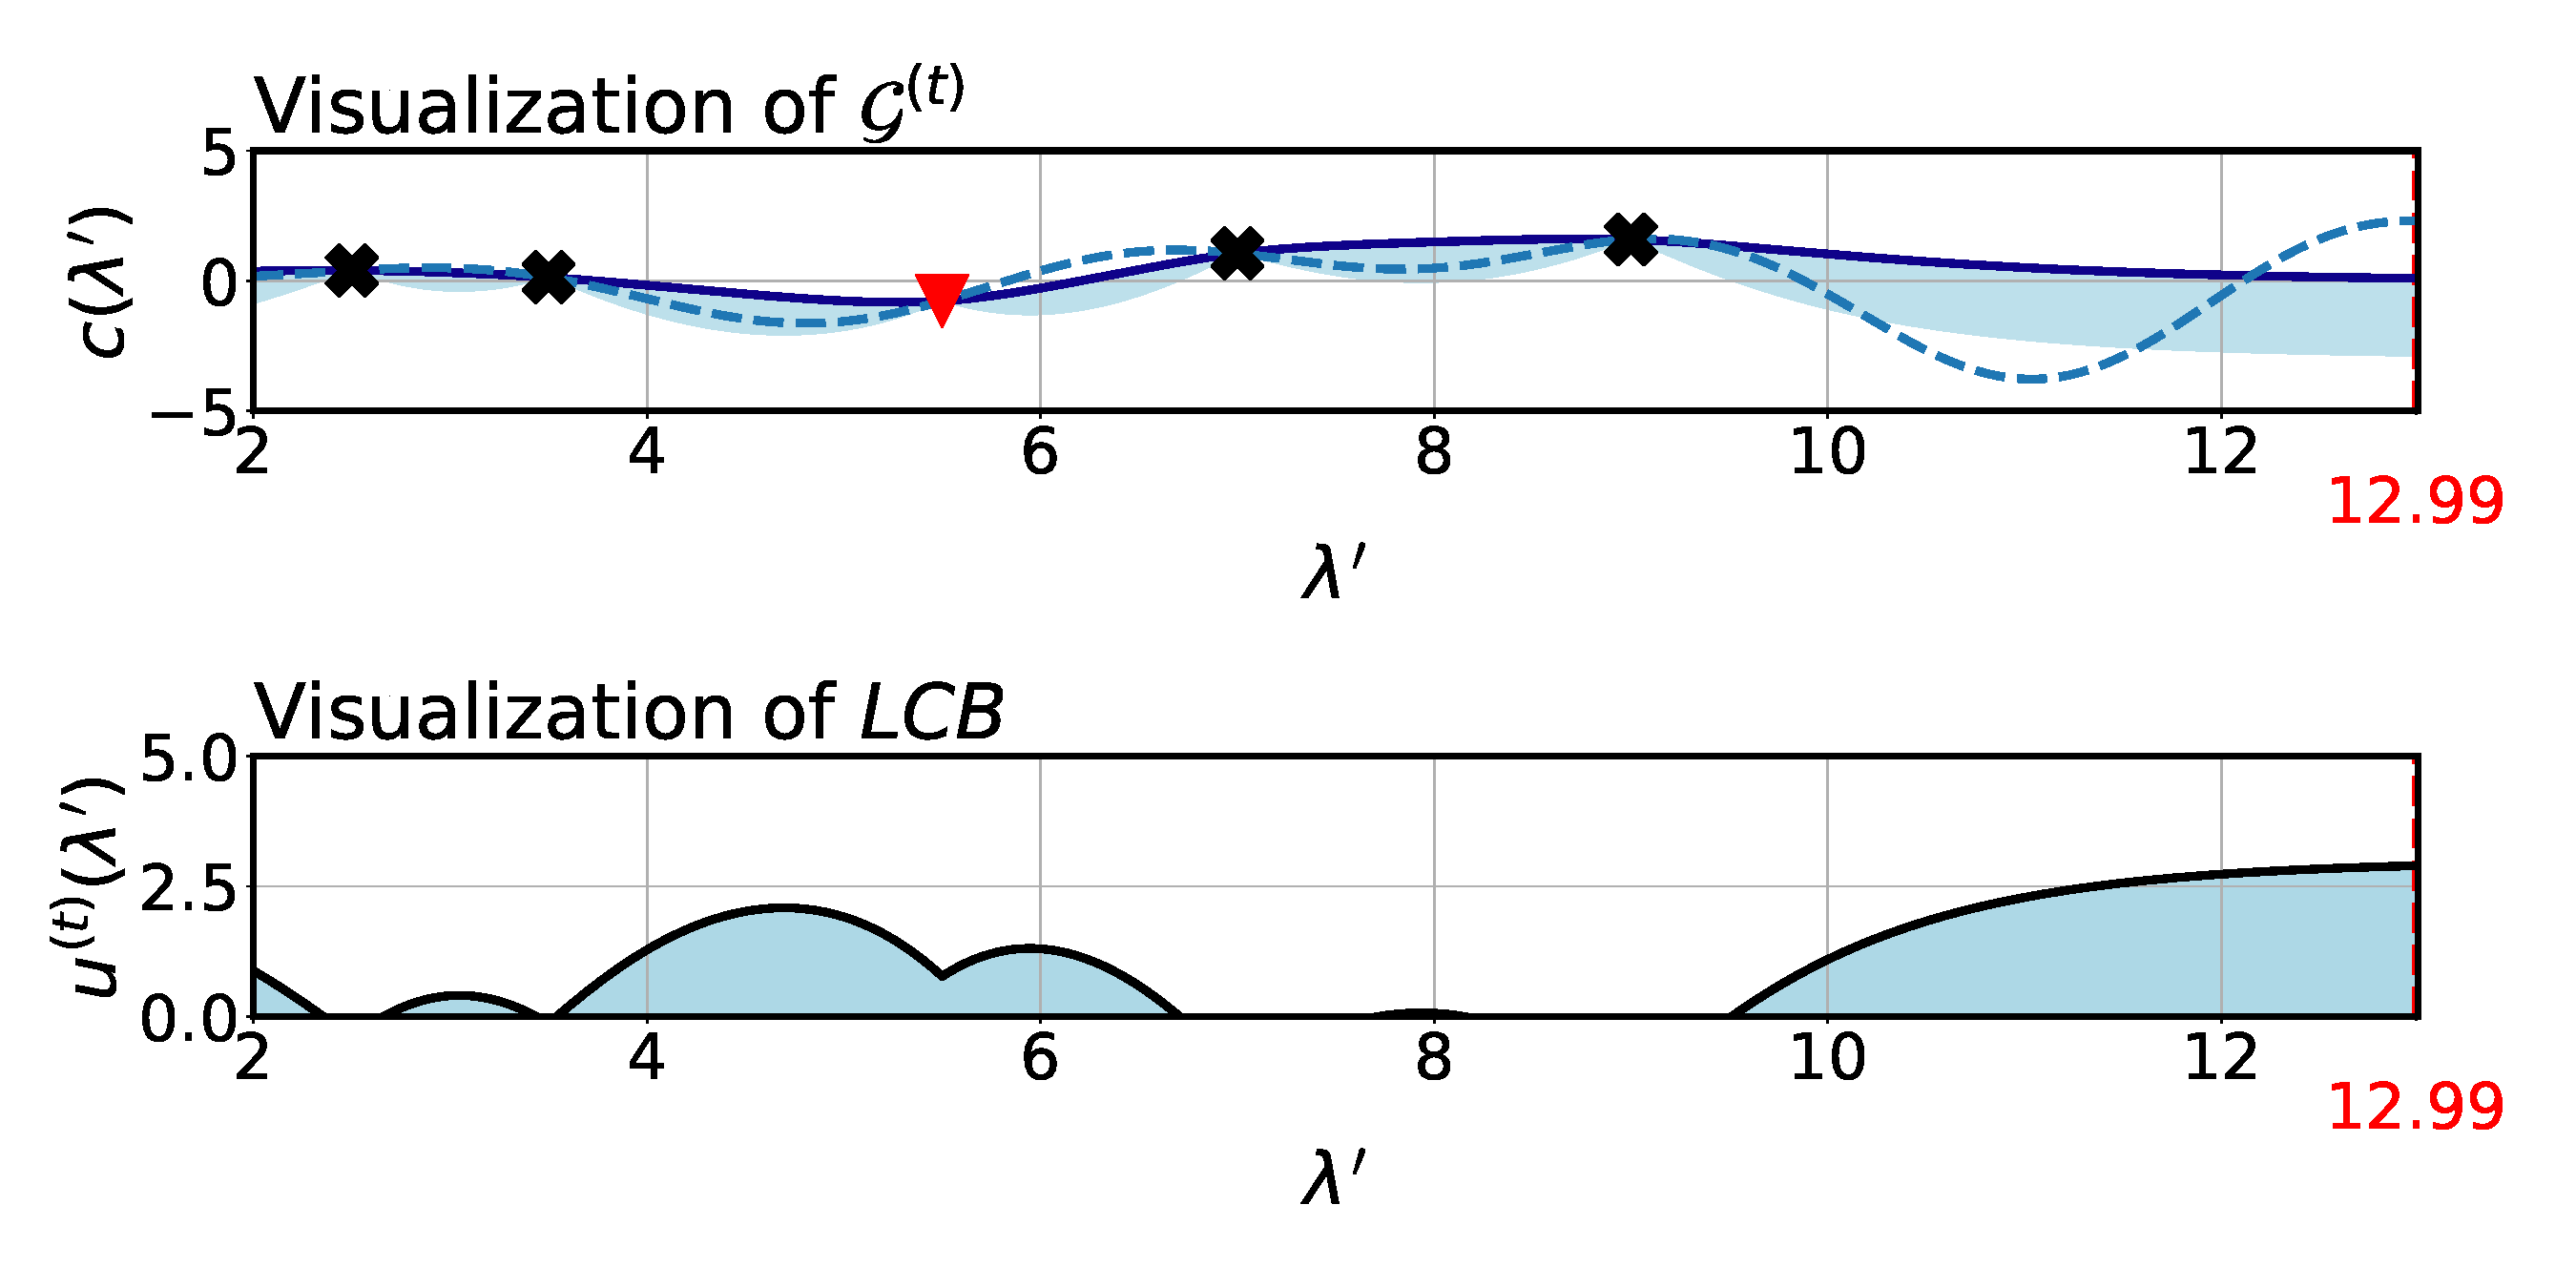
\includegraphics[width=\linewidth, height=0.7\textheight, keepaspectratio=true]{images/acq_func_images/lcb/lcb_3.pdf}};
    \node<.> [below=-1.\belowcaptionskip of img3, align=center]{Pay attention that we \emph{minimize} costs (top) and \\\emph{maximize} the acquisition function (bottom)};
    \node<+> (img4) {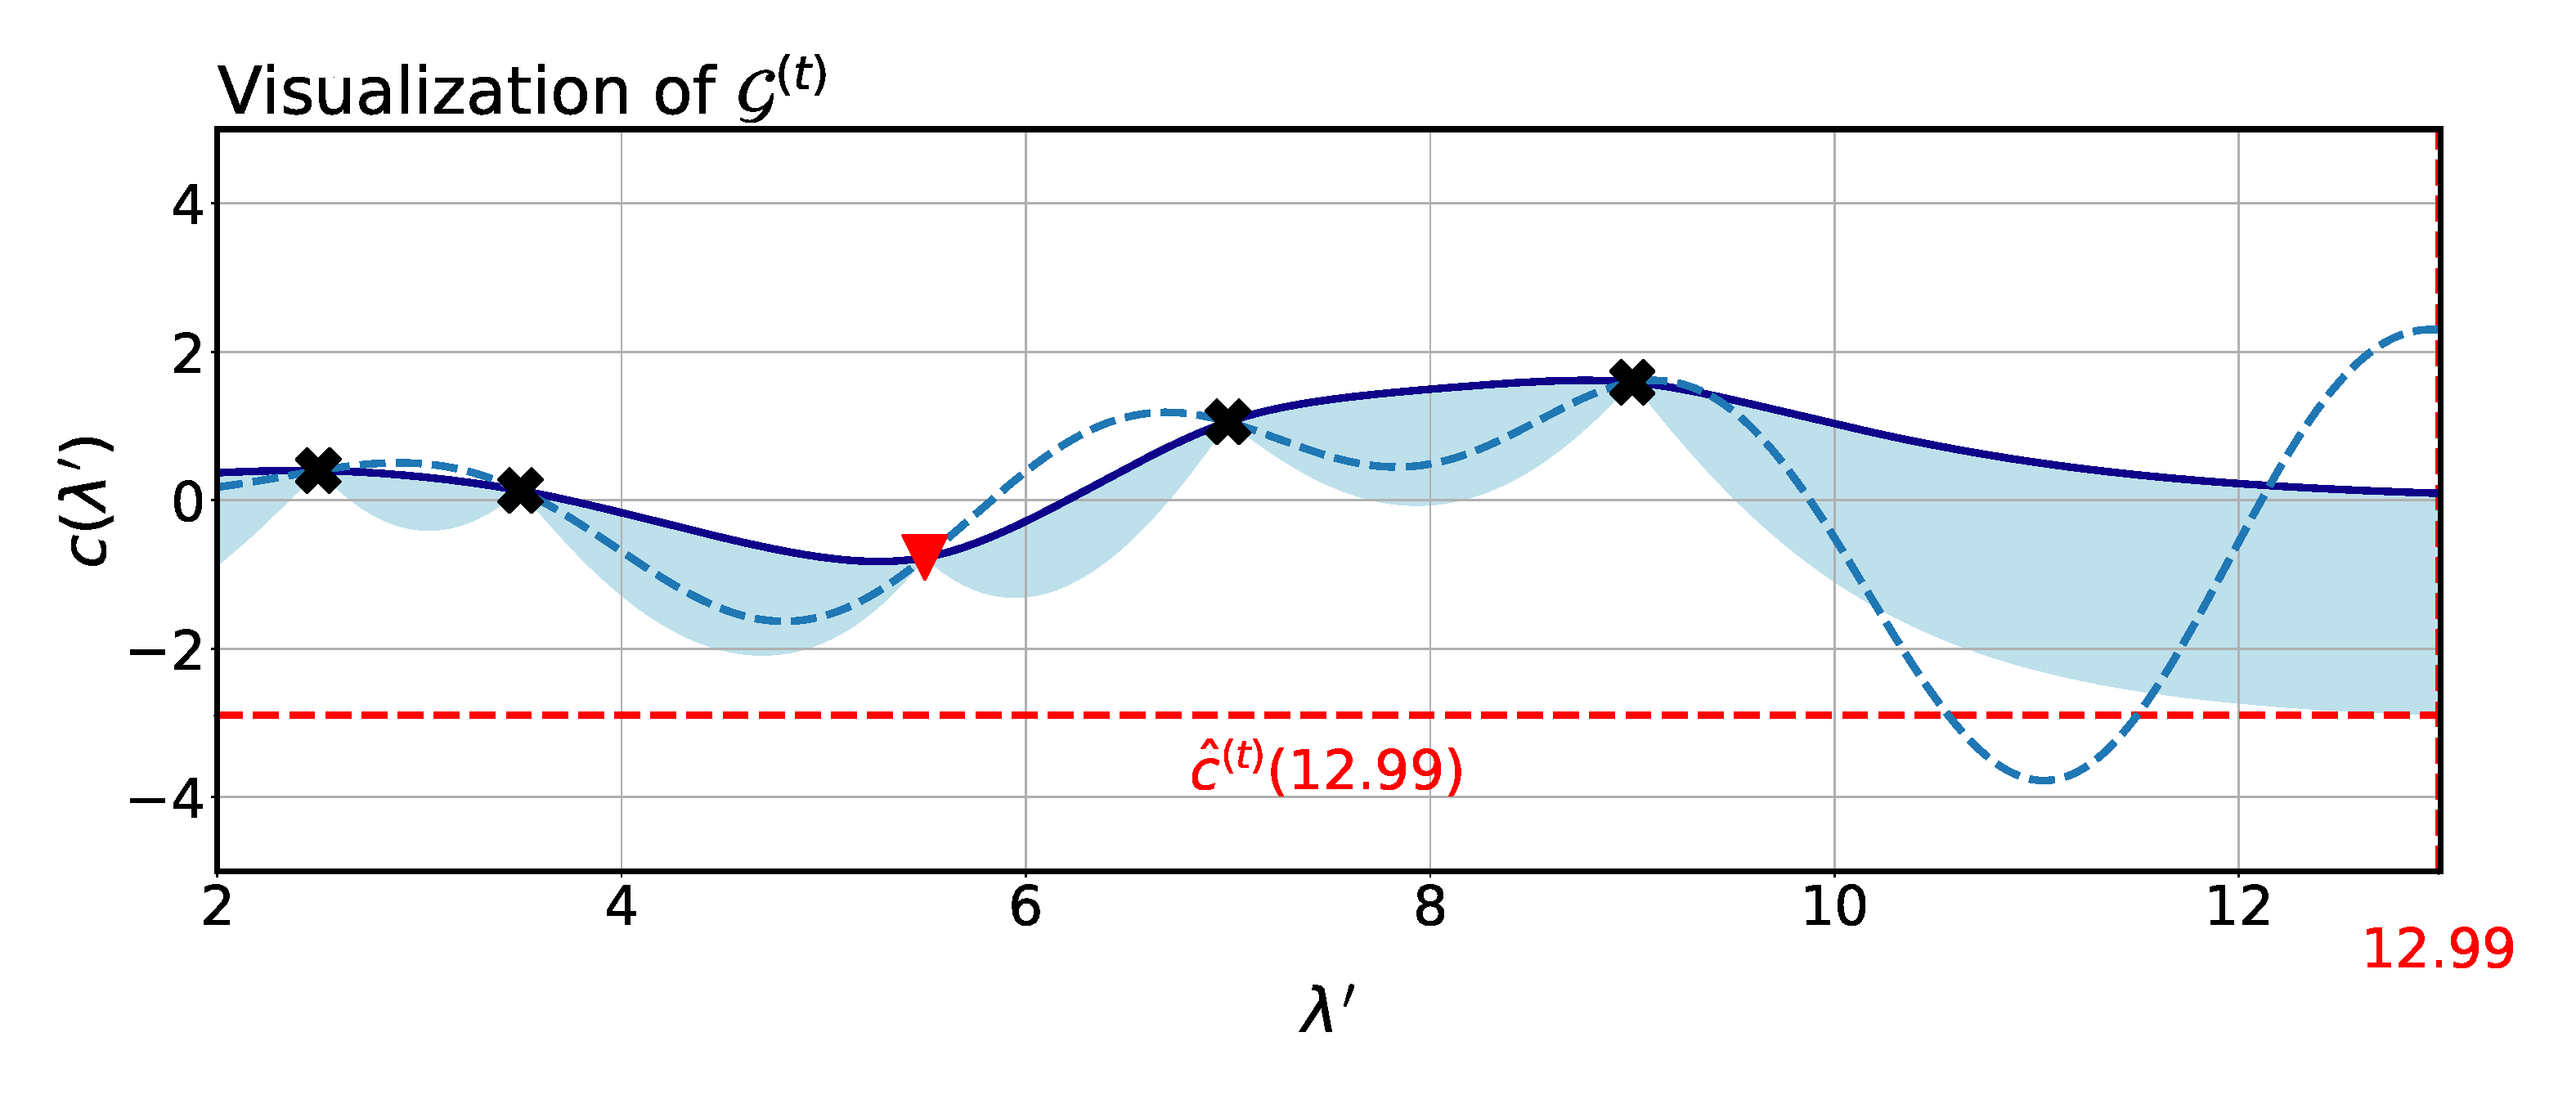
\includegraphics[width=\linewidth, height=0.7\textheight, keepaspectratio=true]{images/acq_func_images/lcb/lcb_4.pdf}};
    \node<.> [below=0.01\belowcaptionskip of img4, align=center]{We choose $\bonextsample=\argmax(LCB(\conf))$};
  \end{tikzpicture}
\end{figure}

\end{frame}
%-----------------------------------------------------------------------
\begin{frame}[c]{Computationally Cheap Acquisition Functions - LCB/UCB}
\framesubtitle{Confidence Bounds - Choosing a candidate}
\begin{itemize}
    \item<+->{We define the Lower Confidence Bound as 
    \[\iter{\acq}_{LCB}(\conf) = \iter{\mean}(\conf) - \alpha\iter{\stddev}(\conf),\quad\alpha\geq0\]}
    \item<+->{It has been shown that using the acquisition function
    \[\iter{\acq}_{GP-LCB}(\conf) = \iter{\mean}(\conf) - \sqrt{\nu\tau_t}\iter{\stddev}(\conf), \quad\nu>0,\] asymptotically results in zero cumulative regret with the appropriate choice of parameters $\tau$ and $\nu$ \lit{\href{https://arxiv.org/pdf/0912.3995.pdf}{Srinivas et al. 2009}}.}
    \comment{Trying to further explain the difference between LCB and GP-LCB's parameters would've overwhelmed the intuitiveness of the slide. Instead, a quick verbal note on the difference and pointing out the reference paper by Srinivas et al. for further reading should suffice.}
    %\comment{Source: Tutorial by Brochu et al.: https://arxiv.org/pdf/1012.2599.pdf }
\end{itemize}
\end{frame}
%-----------------------------------------------------------------------
\begin{frame}[t]{Computationally Cheap Acquisition Functions - TS}
\framesubtitle{Thompson Sampling - Concept}

\begin{figure}
  \centering
  \begin{tikzpicture}
    \node<+> (img1) {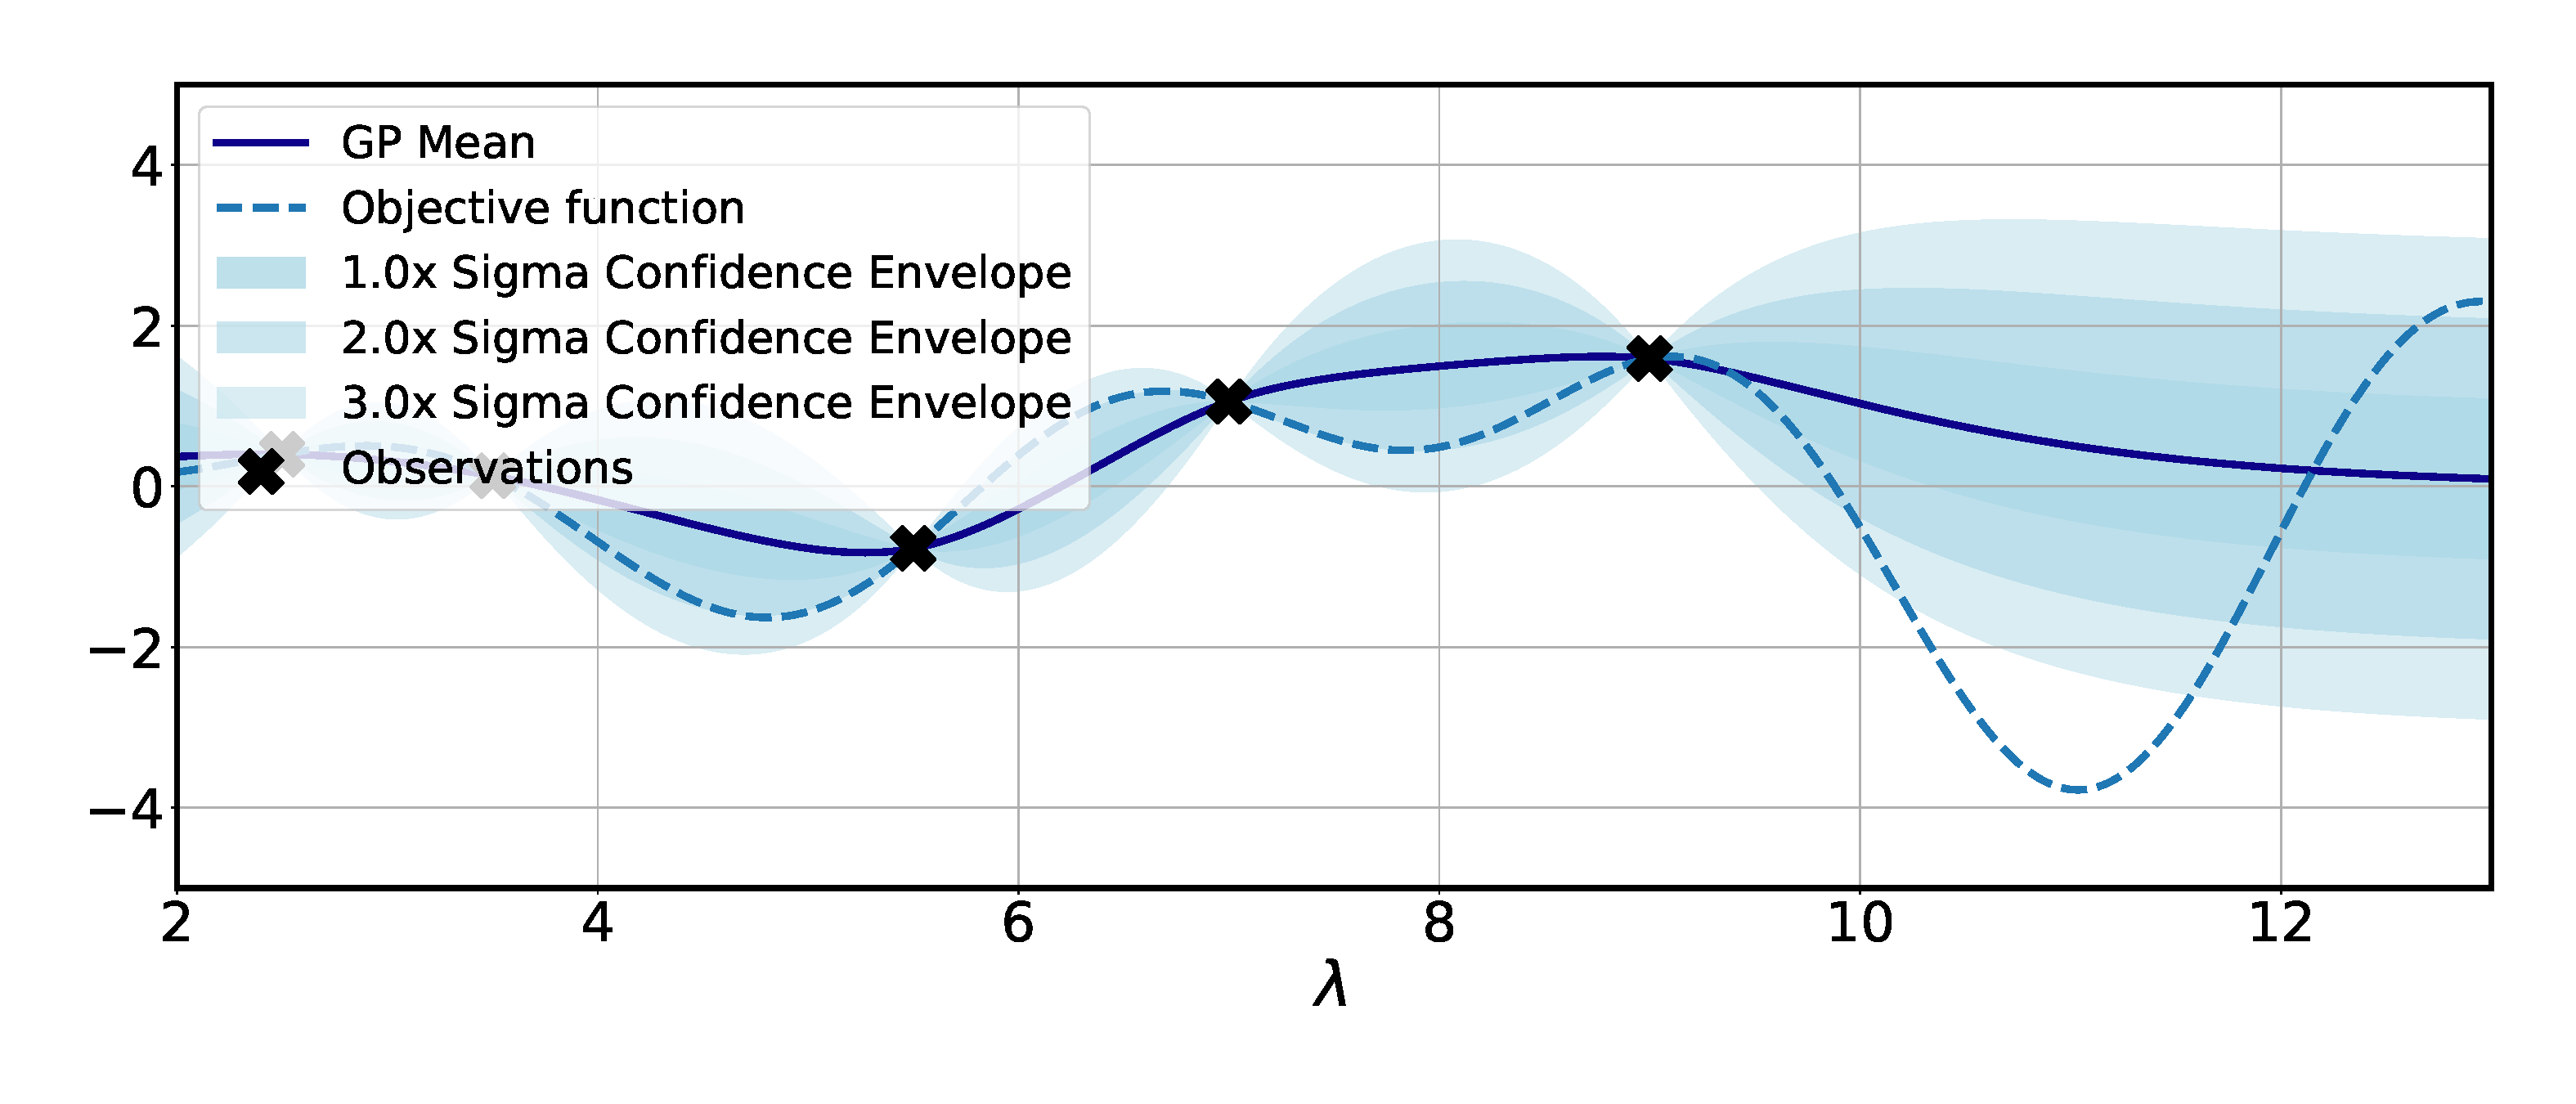
\includegraphics[width=\linewidth, height=0.7\textheight, keepaspectratio=true]{images/acq_func_images/ts/ts_1.pdf}};
    \node<.> [below=0.01\belowcaptionskip of img1, align=center]{Given the GP at iteration $\bocount$ fit on dataset $\iter[\bocount-1]{\dataset}$};
    \node<+> (img2) {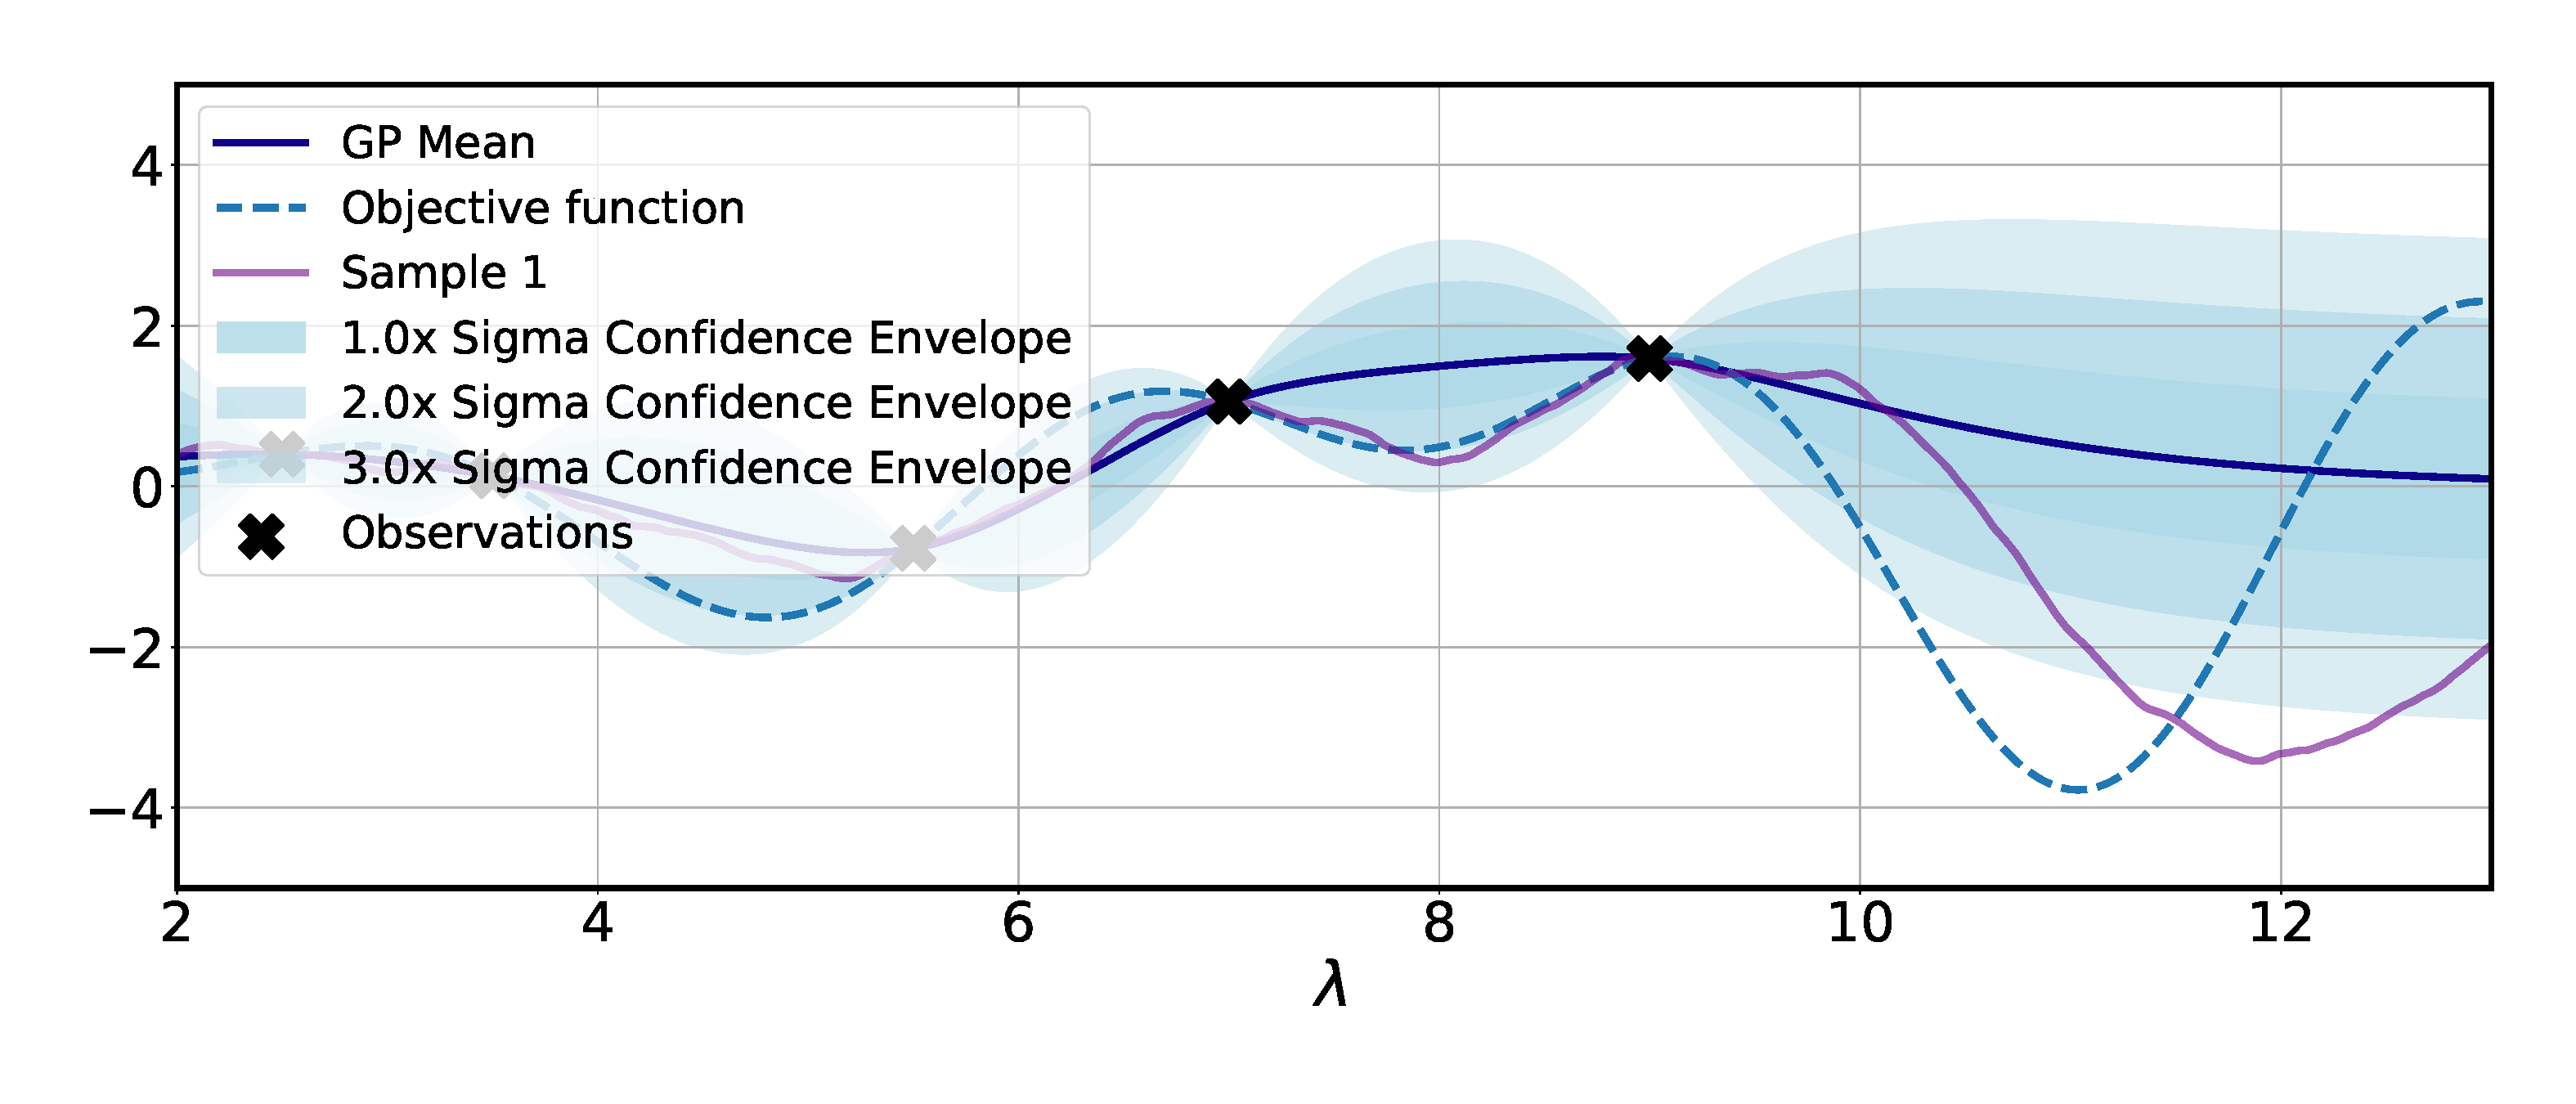
\includegraphics[width=\linewidth, height=0.7\textheight, keepaspectratio=true]{images/acq_func_images/ts/ts_2.pdf}};
    \node<.> [below=0.01\belowcaptionskip of img2, align=center]{Draw a sample $g$ from the GP};
    \node<+> (img3) {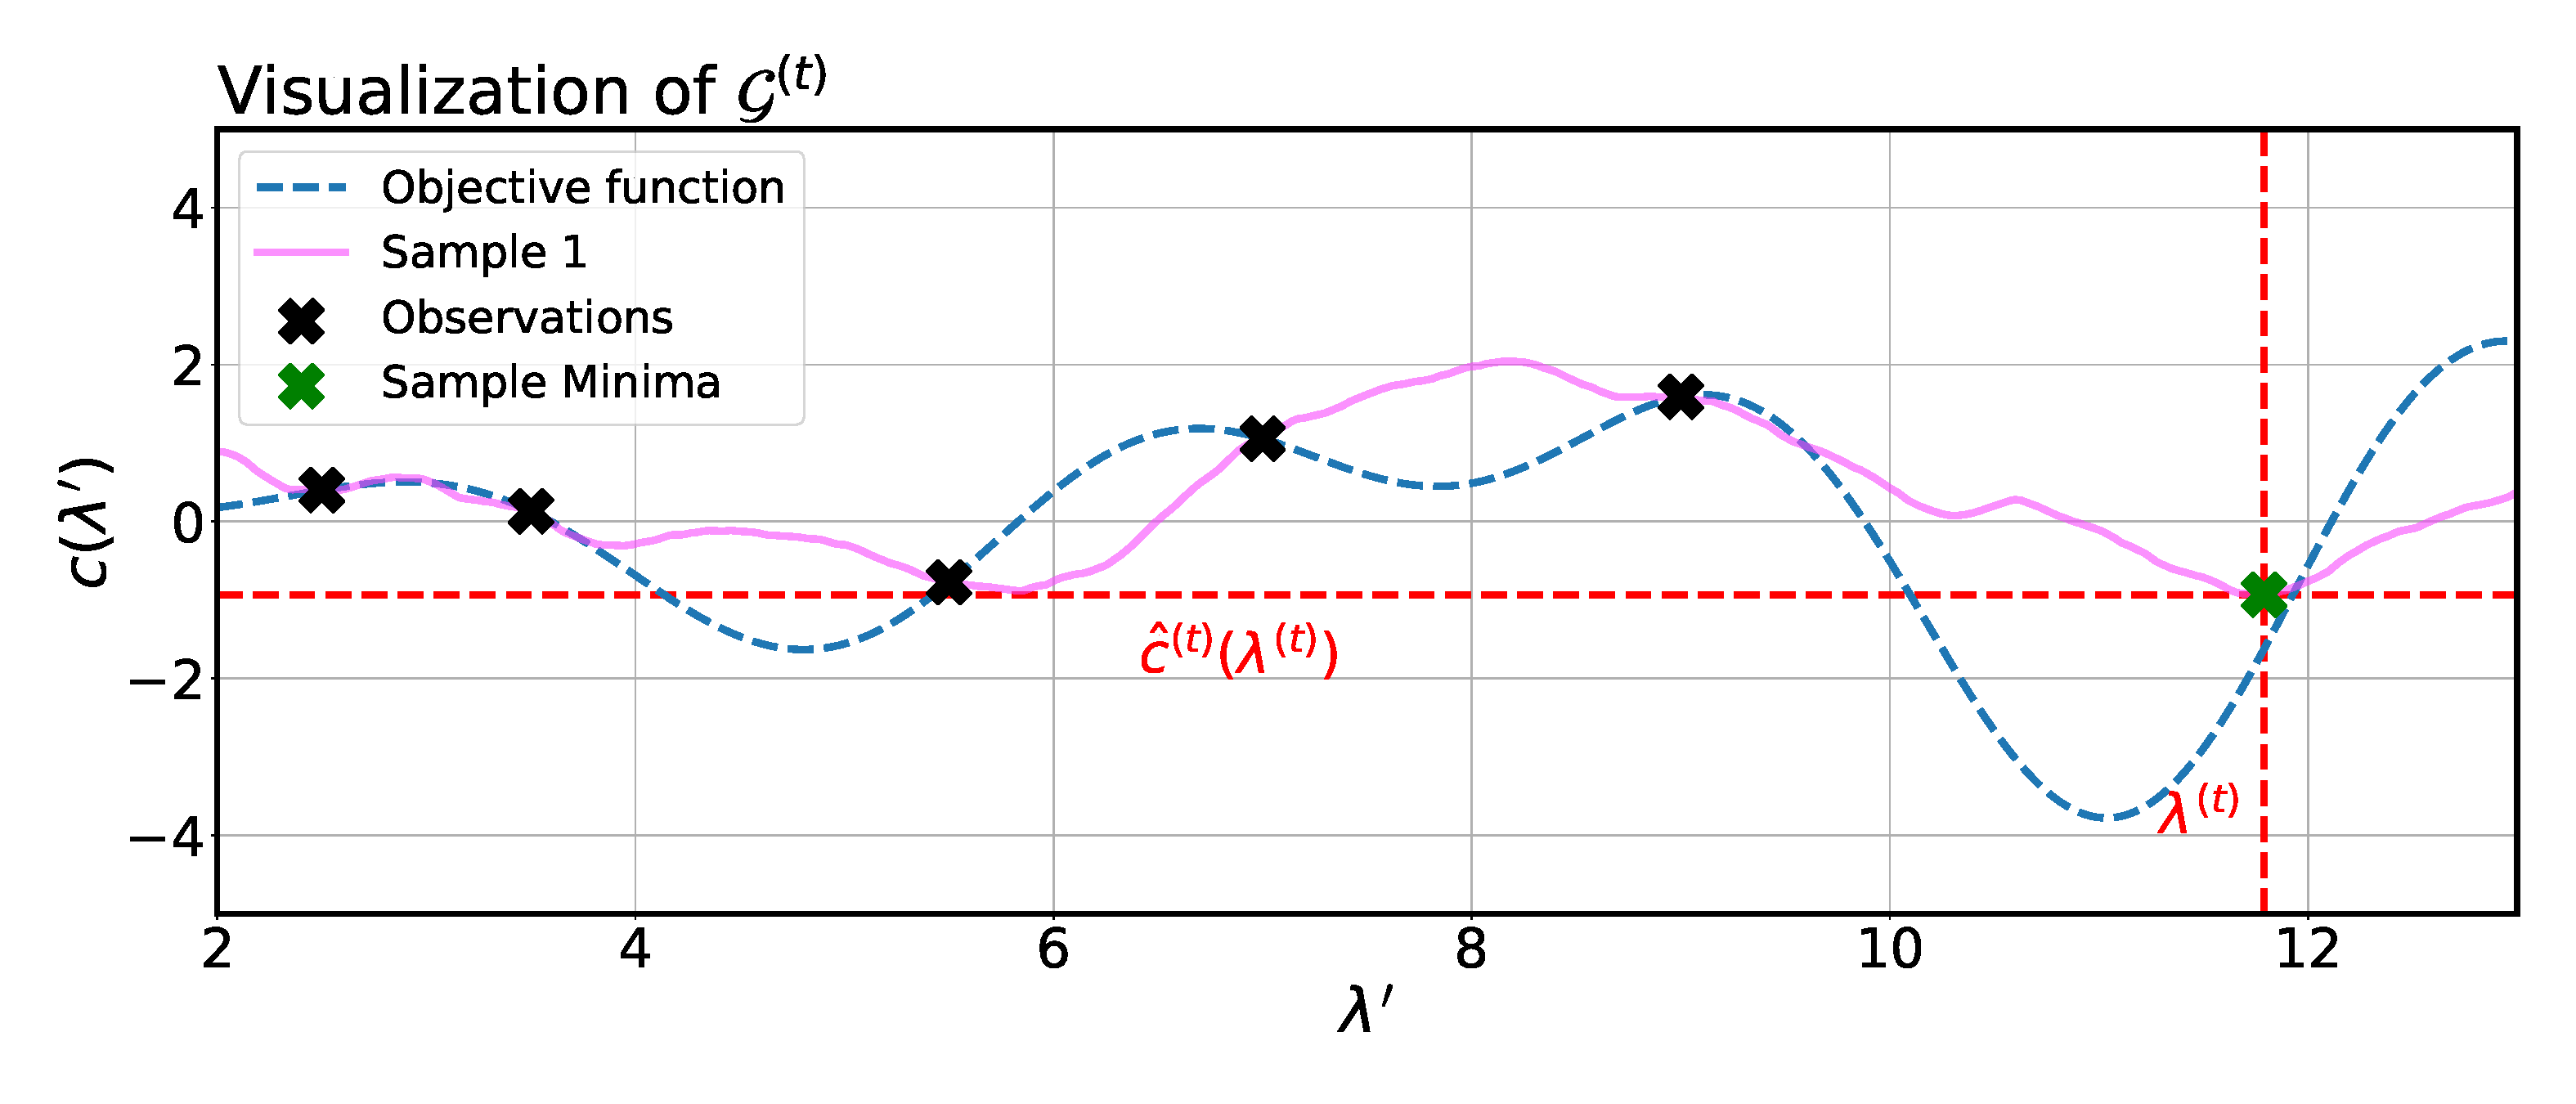
\includegraphics[width=\linewidth, height=0.7\textheight, keepaspectratio=true]{images/acq_func_images/ts/ts_3.pdf}};
    \node<.> [below=0.01\belowcaptionskip of img3, align=center]{Then choose the minimum of this sample to evaluate at next};
    % \node<+> (img4) {\includegraphics[width=\linewidth, height=0.7\textheight, keepaspectratio=true]{images/acq_func_images/ts/ts_4.pdf}};
    % \node<.> [below=0.01\belowcaptionskip of img4, align=center]{Then choose the minimum of this sample};
  \end{tikzpicture}
\end{figure}

\end{frame}
%-----------------------------------------------------------------------
% \begin{frame}[c]{Computationally Cheap Acquisition Functions - TS}
% \framesubtitle{Thompson Sampling - Gist}
% 
% \begin{itemize}
%     \item Draw a sample $g$ from the GP $\iter{\gp}$.
%     \item Choose $\bonextsample=\argmin_{\conf\in\pcs}(g(\conf))$
% \end{itemize}
% \end{frame}
%-----------------------------------------------------------------------
\begin{frame}[c]{Computationally Cheap Acquisition Functions - TS}
\framesubtitle{Thompson Sampling - Choosing a candidate}
\begin{center}
\begin{minipage}{0.75\textwidth}
\comment{Fix algorithm numbering}
\begin{algorithm}[H]
    %\DontPrintSemicolon
    \LinesNumbered
    \SetAlgoLined
    \setcounter{AlgoLine}{0}
    \SetKwInOut{Require}{Require}
    \SetKwInOut{Result}{Result}
    
    \Require{Search space $\pcs$, 
    		cost function $\cost$, 
    		Gaussian process $\gp$,
    		maximal number of function evaluations $\bobudget$}
\Result{Best observed configuration $\finconf$ according to $\iter[\bobudget]{\dataset}$ or $\gp$}    
    $\iter[0]{\dataset}\leftarrow\varnothing$\;
    
    \For{$\bocount=1$ \KwTo $\bobudget$}{
    
        $\iter[\bocount]{\gp}$ $\leftarrow$ fit \textcolor{blue}{Gaussian process} on $\iter[\bocount-1]{\dataset}$\;
    
        \textcolor{blue}{Sample $g\sim\iter{\gp}$}\;
    
        \textcolor{blue}{$\bonextsample\leftarrow \bonextsample \in \argmin_{\conf\in\pcs}g(\conf)$}\;
    
        Query $\bonextobs$\;

    	$\iter[\bocount]{\dataset} \leftarrow \iter[\bocount-1]{\dataset} \cup \{\langle \bonextsample, \bonextobs \rangle \}$\;
        }
    \caption{Bayesian Optimization using Thompson Sampling}
\end{algorithm}
\end{minipage}
\end{center}
%\comment{Source: Paper, Kandasamy et al, http://proceedings.mlr.press/v84/kandasamy18a/kandasamy18a.pdf}
\end{frame}
%-----------------------------------------------------------------------
\begin{frame}[c]{Questions to Answer for Yourself / Discuss with Friends}

\begin{itemize}
%PI
    \item \emph{Discussion.} How would you set the exploration parameter $\xi$ for PI in practice?
%EI
    \item \emph{Derive.} Starting from the improvement over the current incumbent, derive the closed form solution of expected improvement.
    \item \emph{Discussion.} In which situations would EI perform substantially different than PI?
%LCB
%TS
\end{itemize}

\end{frame}